
%
% foundations
%

\chapter{Foundations}
\label{chapter:foundations}

In the following chapter, the technical foundations of cluster theory, computing spatial data and fundamental concepts of web mapping are explained. The definition of the clustering task, an overview cluster analysis history as well as basic definitions of cluster types, clustering techniques and proximity measures are given. Four foundational clustering algorithms are explained to provide an overview and understanding of the basic differentiation between clustering techniques. Approaches for dealing with spatial data are laid out by discussing space order methods, space decomposition methods, Quadtrees and the Geohash encoding.


%
% foundations - clustering
%

\section{Clustering}

Clustering is the task of grouping unlabeled data in an automated way. It can also be described as the unsupervised classification of patterns into groups. The techniques of cluster analysis are applied in numerous scenarios including data mining, document retrieval, image segmentation and pattern classification. They are used to solve different tasks including pattern-analysis, grouping, decision-making or machine-learning.

Cluster analysis has been studied since the early beginnings of computer science and applies to a broad number of research fields. Different research communities have created a variety of vocabularies to describe methods related to clustering. Analog to the term cluster analysis, other names are used in literature: Q-analysis, topology, grouping, comping, classification, numerical taxonomy and unsupervised pattern recognition.

As indicated, clustering is a wide and generic term. Often it is used to refer to specific concepts which are appropriate for solving specific tasks. This means that efficient clustering algorithms have been developed and studied over the years for certain research fields. While such algorithms might perform well under certain circumstances, they might be completely inappropriate for other use cases. Imagine, an algorithm that  fits image segmentation well but is less useful in machine-learning~\cite{Meert06clustermaps, Jain99clusterreview}.

Clustering is a general concept that applies to multivariate data. Spatial data in this sense is a special case, and 2-dimensional spatial data reduces the problem space even further to planar space. Figure~\ref{fig:clusters} visualizes such an example of clusters of point patterns in two dimensional space. Humans can understand and perform this kind of clustering tasks competitively whereas clustering in high-dimensional space is difficult for humans to obtain. 

\begin{figure}[h]
  \begin{center}
    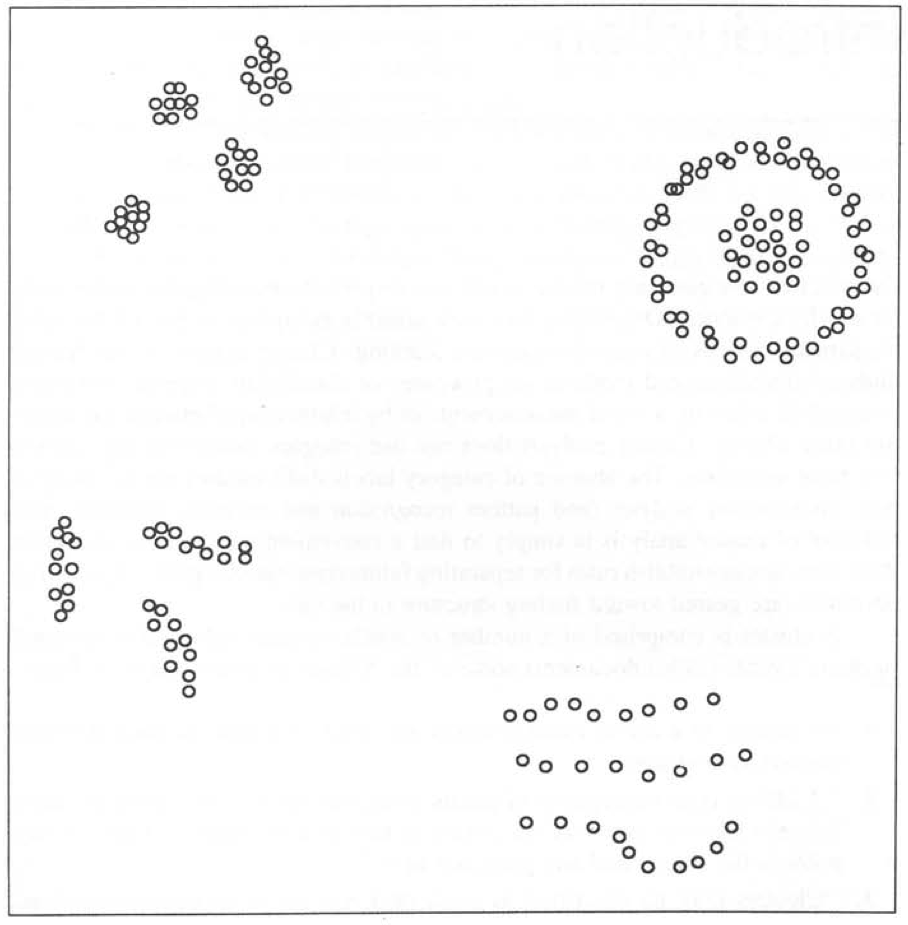
\includegraphics[width=0.75\textwidth]{figures/clusters.png}
    \caption{Clusters of point patterns in two dimensions~\cite[p 2]{Jain99clusterreview}.}
    \label{fig:clusters}
  \end{center}
\end{figure}



\subsection{The Clustering task}

Clustering is the task of aggregating items (also described as features) into clusters, based on similarities or proximity. A.K. Jain, M.N. Murty and P.J. Flynn~\cite{Jain99clusterreview} define the following steps involved in a typical pattern clustering activity:
 
\begin{quote}
\begin{enumerate}
\item pattern representation (optionally including feature extraction and/or selection), 
\item definition of a pattern proximity measure appropriate to the data domain, 
\item clustering or grouping, 
\item data abstraction (if needed), and 
\item assessment of output (if needed). 
\end{enumerate}
\end{quote}



\subsection{History}

K-means, one of the oldest and most widely used clustering algorithm was introduced already in 1967~\cite{MacQueen67kmeans, Meert06clustermaps}. Tryon and Bailey (1970) wrote one of the first books on cluster analysis. In 1973, Anderberg published ``Cluster analysis for applications'', a book that Jain and Dubes describe as ``the most comprehensive book for those who want to use cluster analysis''~\cite{Jain88clustering}.  While Tryon and Bailey focus on a single clustering approach (BC TRY), Anderberg already gives a comprehensive overview of clustering methods, strategies and a comparative evaluation of cluster analysis methods.

Clustering algorithms were improved and developed further over time, i.e. to account for performance issues. Prominent algorithms in that area include CLARANS~\cite{Ng94CLARANS} and BIRCH~\cite{Zhang96BIRCH} - they have a time complexity linear in the number of patterns. A popular, density based clustering algorithm is DBSCAN~\cite{Ester96DBSCAN}. Jain and Dubes summarize hierarchical and partitional clustering approaches in ``Algorithms for Clustering Data'' (1988) with a special focus on applications in image processing. Numerous subsequent publications on cluster analysis are released continuously~\cite{Jain99clusterreview}. 



\subsection{Cluster types}

Clusters are groupings of similar objects. Different models of interpretations of clusters exist: most notably, they can be classified into different types of clusters:

\begin{itemize}

\item \textbf{Well-separated} clusters have the property that objects within a cluster are closer to each other than any object outside of the cluster. As the name suggests, this is only possible when the data contains natural clusters that are quite far from each other.

\item \textbf{Prototype-based} clusters are defined so that objects are closer to their cluster's prototype than to any other one. Prototypes of clusters are either centroids (the mean of all points for a cluster) for continuous data or medoids (the most central point within a cluster) for categorical data.

\item \textbf{Graph-based} clusters can be defined as \emph{connected components} within a graph. That is a group of objects (nodes) where the objects are connected to one another but disconnected from objects outside of the cluster.

\item \textbf{Density-based} clusters group objects within dense regions that are surrounded by a region of low density. Such a definition is often employed when noise is present or clusters are irregular~\cite{Meert06clustermaps}.

\end{itemize}

\begin{figure}[h]
  \begin{center}
    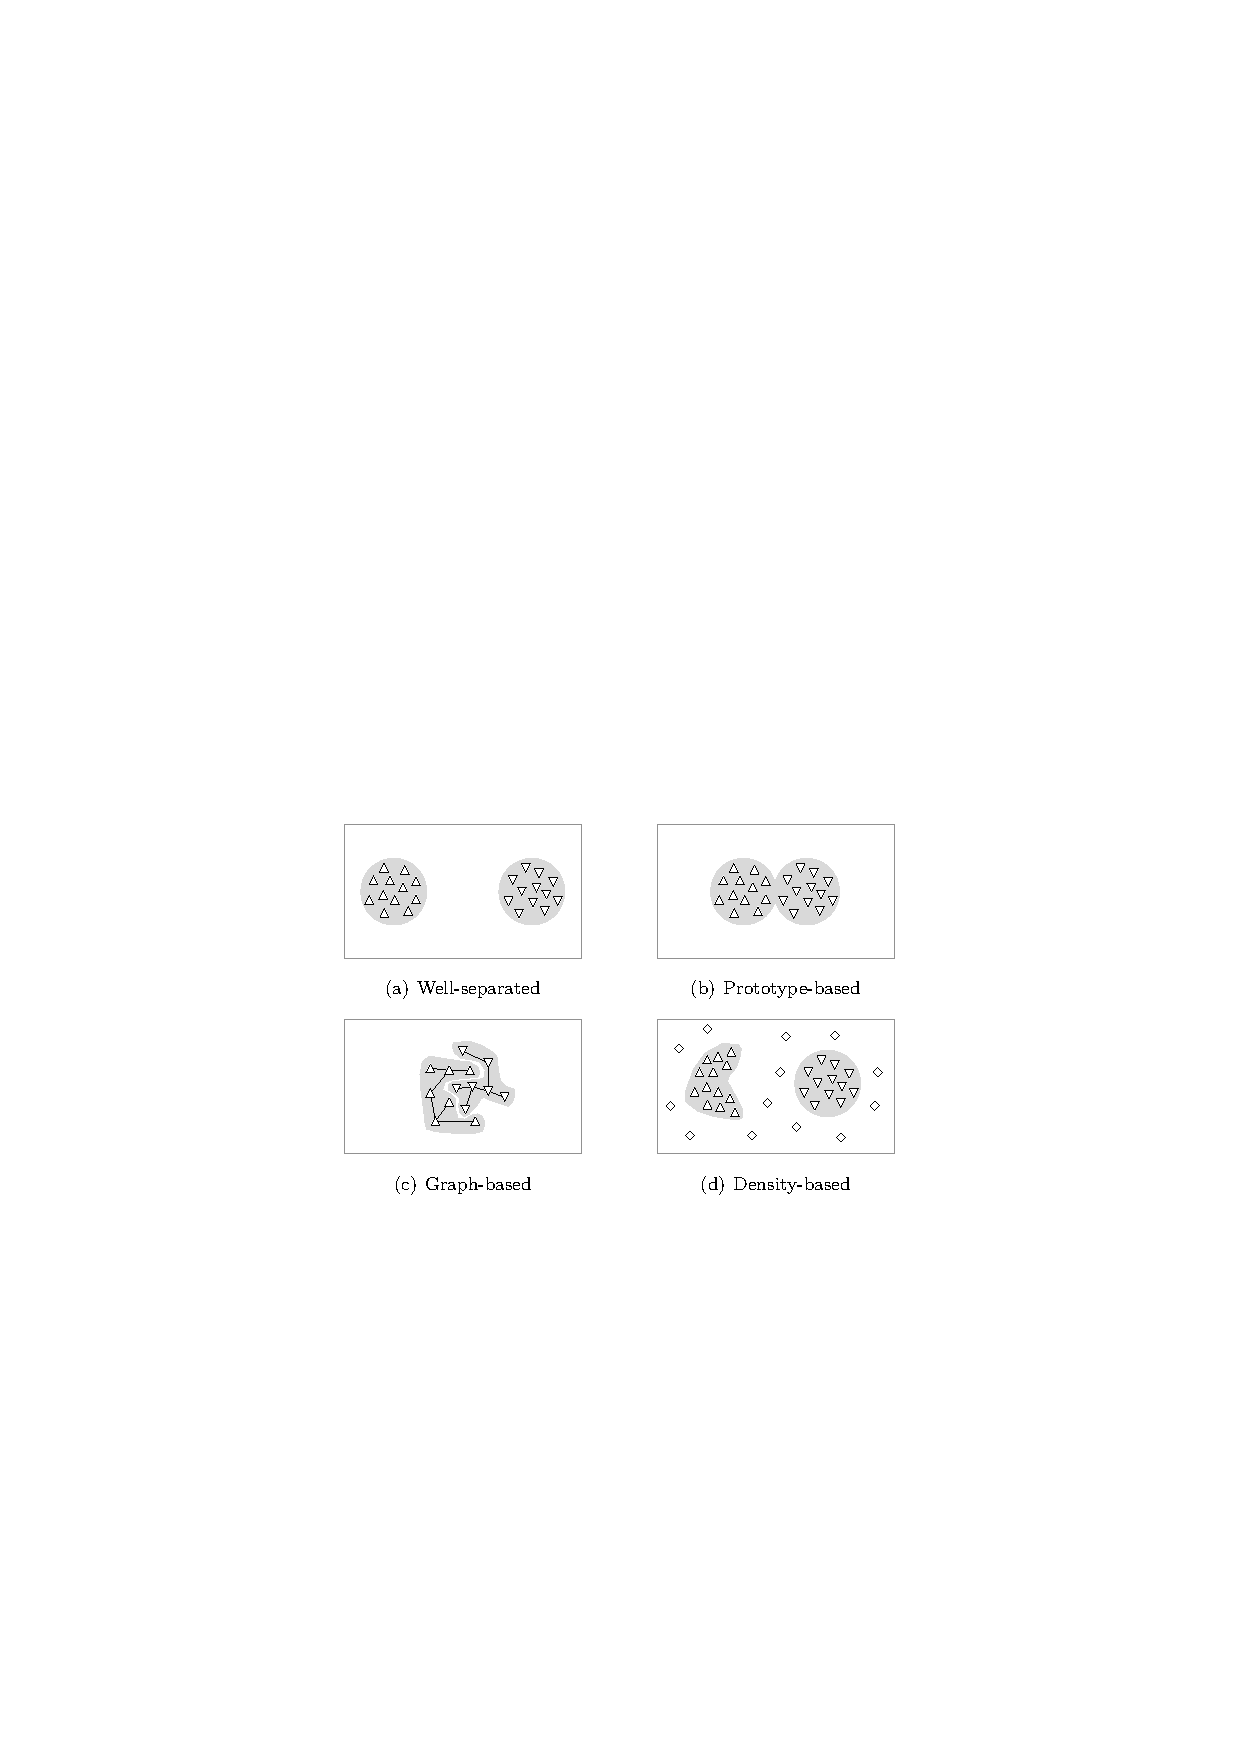
\includegraphics[width=0.75\textwidth]{figures/cluster_types.pdf}
    \caption{Types of clusters: (a) Well-separated, (b) Prototype-based, (c) Graph-based, (d) Density-based~\cite[p 9]{Meert06clustermaps}.}
    \label{fig:clusters}
  \end{center}
\end{figure}



\subsection{Clustering techniques}
\label{chapter:clustering-techniques}

Literature research reveals classifications of clustering techniques according to various aspects. Jain, Murty and Flynn primarily group the algorithms into hierarchical and partitional ones~\cite{Jain99clusterreview}. On the other hand, Stein and Busch split them into hierarchical, iterative, density-based and meta-search-controlled~\cite{Stein05density}. The differentiation of properties into groupings of clustering techniques and cross-cutting aspects is inconsistent among publications. This again shows the wide variety in which cluster analysis is being discussed and developed.

\begin{figure}[h]
  \begin{center}
    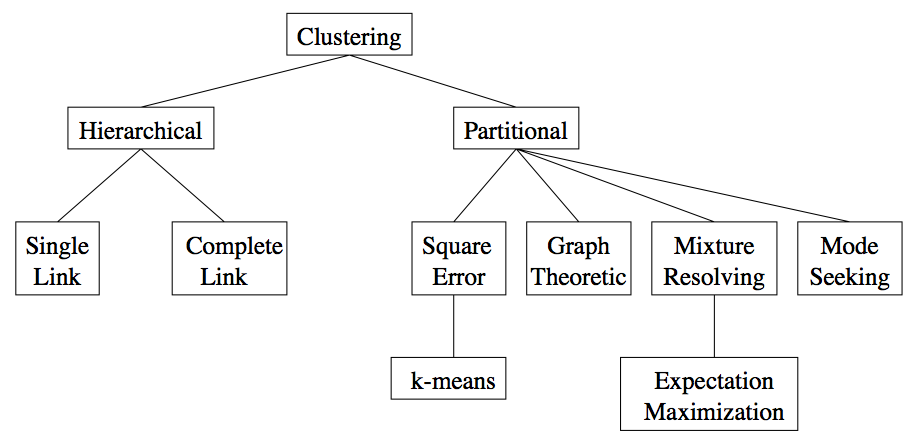
\includegraphics[width=0.9\textwidth]{figures/clustering_approaches_jain.png}
    \caption{A taxonomy of clustering approaches.~\cite[p 275]{Jain99clusterreview}.}
    \label{fig:clusters}
  \end{center}
\end{figure}

\begin{figure}[h]
  \begin{center}
    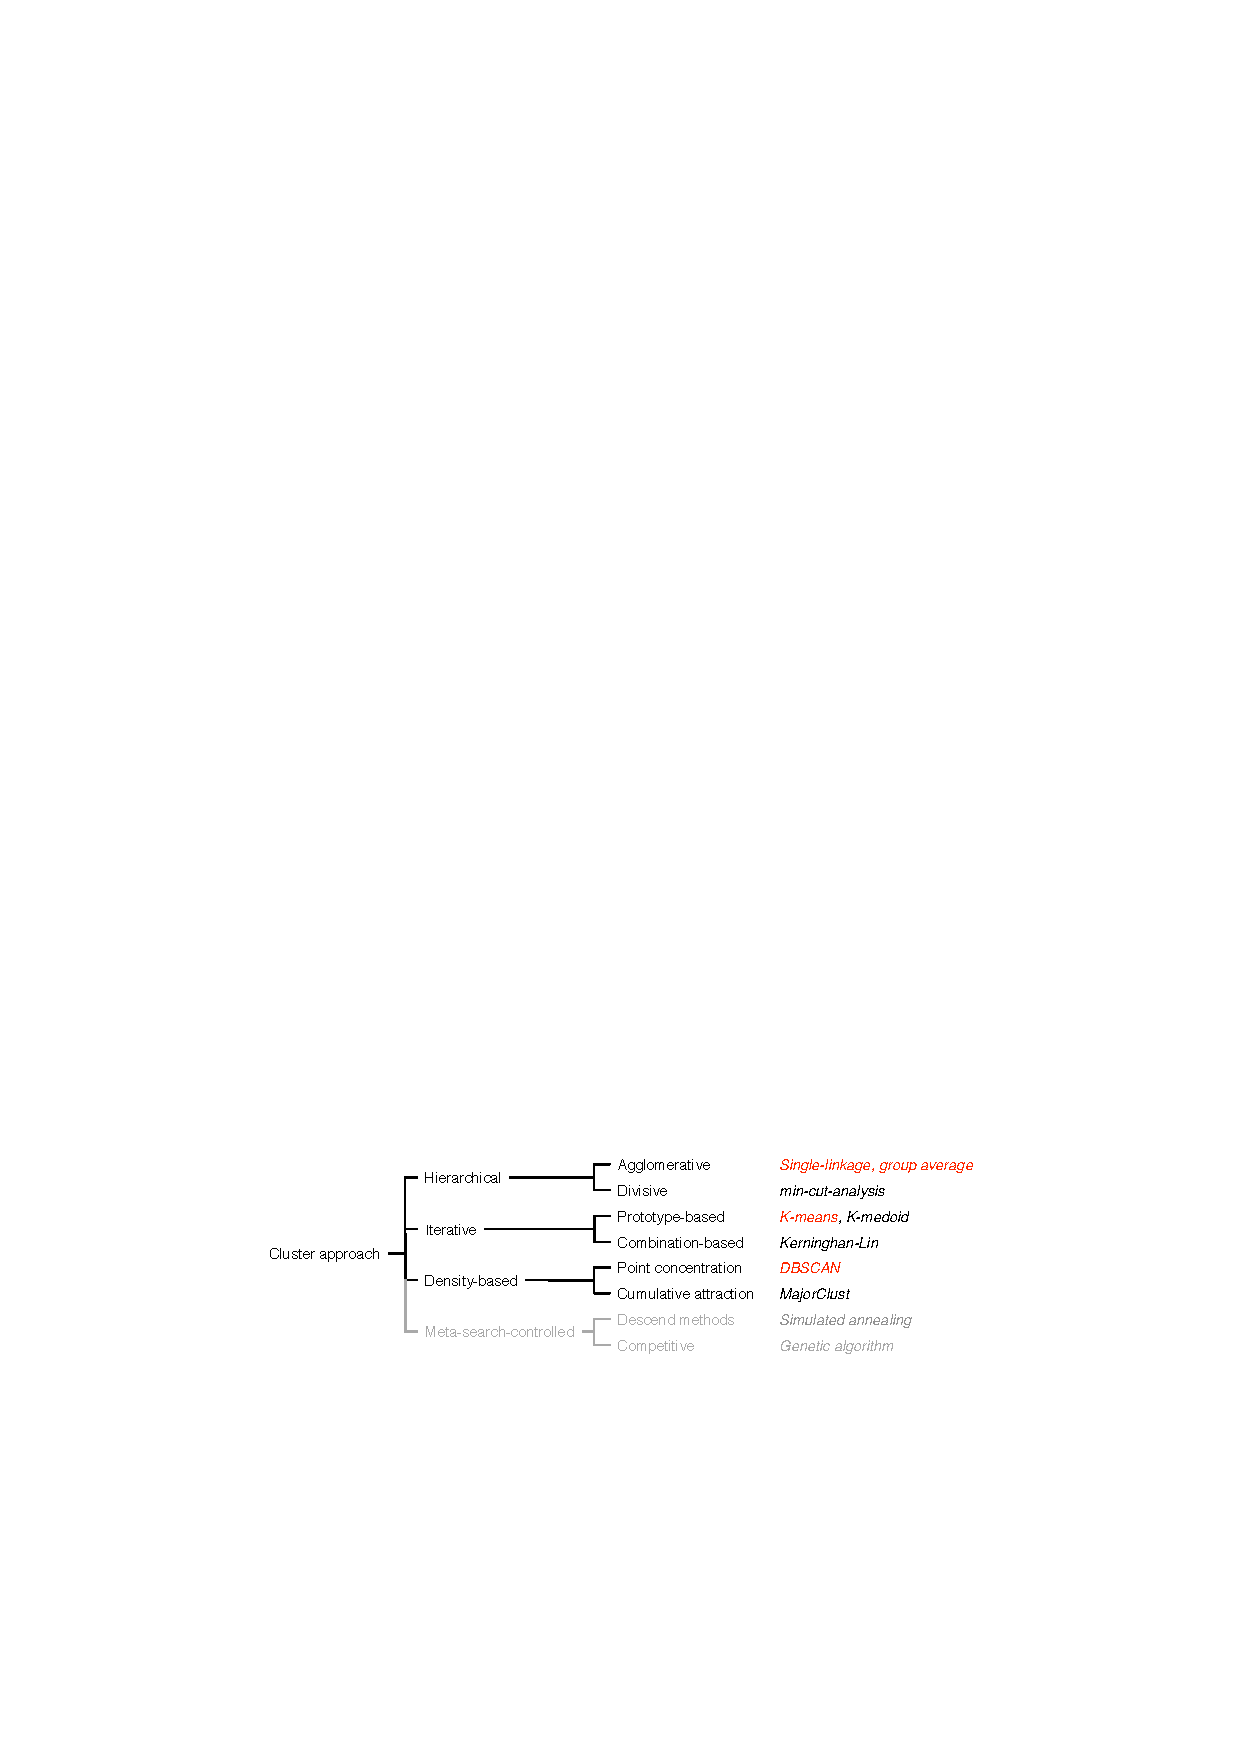
\includegraphics[width=1\textwidth]{figures/clustering_techniques_meert.pdf}
    \caption{A taxonomy of cluster algorithms as cited in~\cite[p 14]{Meert06clustermaps}, based on \cite{Stein05density}.}
    \label{fig:clusters}
  \end{center}
\end{figure}

\begin{itemize}

\item \textbf{Hierarchical versus Partitional}. Whether it is nested is the classic differentiation between clustering techniques. \textit{Partitional clustering} divides the data set into non-overlapping clusters. It usually is driven by an \textit{iterative} approach that optimized the result.
\textit{Hierarchical clustering} organizes clusters as a tree. Each node in the tree is the union of its children. Both clustering types are related: applying partitional clusterings in a sequence can lead to a hierarchical clustering and cutting the hierarchical tree at a particular level produces a partitional clustering~\cite{Meert06clustermaps}. 

An example of the relationship between hierarchical and partitional clustering is given by the following example of density-based algorithms. \textit{DBSCAN} produces simple data partitions and was further developed into \textit{OPTICS} which clusters data hierarchically~\cite{wiki:DBSCAN}.     

\item \textbf{Agglomerative versus divisive}. \textit{Agglomerative clustering} algorithms start with single items and successively merge them together into clusters. On the other hand, \textit{divisive clustering} algorithms begin with a single cluster that contains all items and splits it up until a stopping criterion is met. Each such merging or splitting procedure can be seen as one level in the hierarchical clustering tree~\cite{Jain99clusterreview}.

\item \textbf{Hard versus Fuzzy}. \textit{Hard clustering} algorithms assign every item to a single cluster, this means that the clustering is \textit{exclusive}. A \textit{fuzzy clustering} algorithm may attribute an item to multiple clusters in a \textit{non-exclusive way }by assigning degrees of membership. A fuzzy clustering may be converted into a hard clustering by assigning every data item to the cluster with the highest degree of membership~\cite{Jain99clusterreview, Meert06clustermaps}.

\item \textbf{Complete versus Partial}. With \textit{complete clustering}, assigning every point to a cluster is required. \textit{Partial clustering} relaxes this requirement so that not every point needs to be assigned to a cluster. This can be particularly useful when clustering data sets with outliers and noise. In such cases, the partial clustering can be used to focus on crowded areas~\cite{Jain99clusterreview}. 

\end{itemize}

Further aspects include monothetic versus polythetic and incremental versus non-incremental clustering techniques. 



\subsection{Proximity}
\label{chapter:proximity}

Similarity is fundamental to the definition of a cluster. In order to measure similarity, clustering algorithms evaluate their proximity. Continuous data requires different proximity measurements than categorical data.

For continuos data, the proximity between items is typically quantified by dissimilarity in terms of distance measures. The three main distance functions are visualized in figure~\ref{fig:clustering-proximity} and explained as follows\cite{Meert06clustermaps}:

\begin{figure}[h]
  \begin{center}
    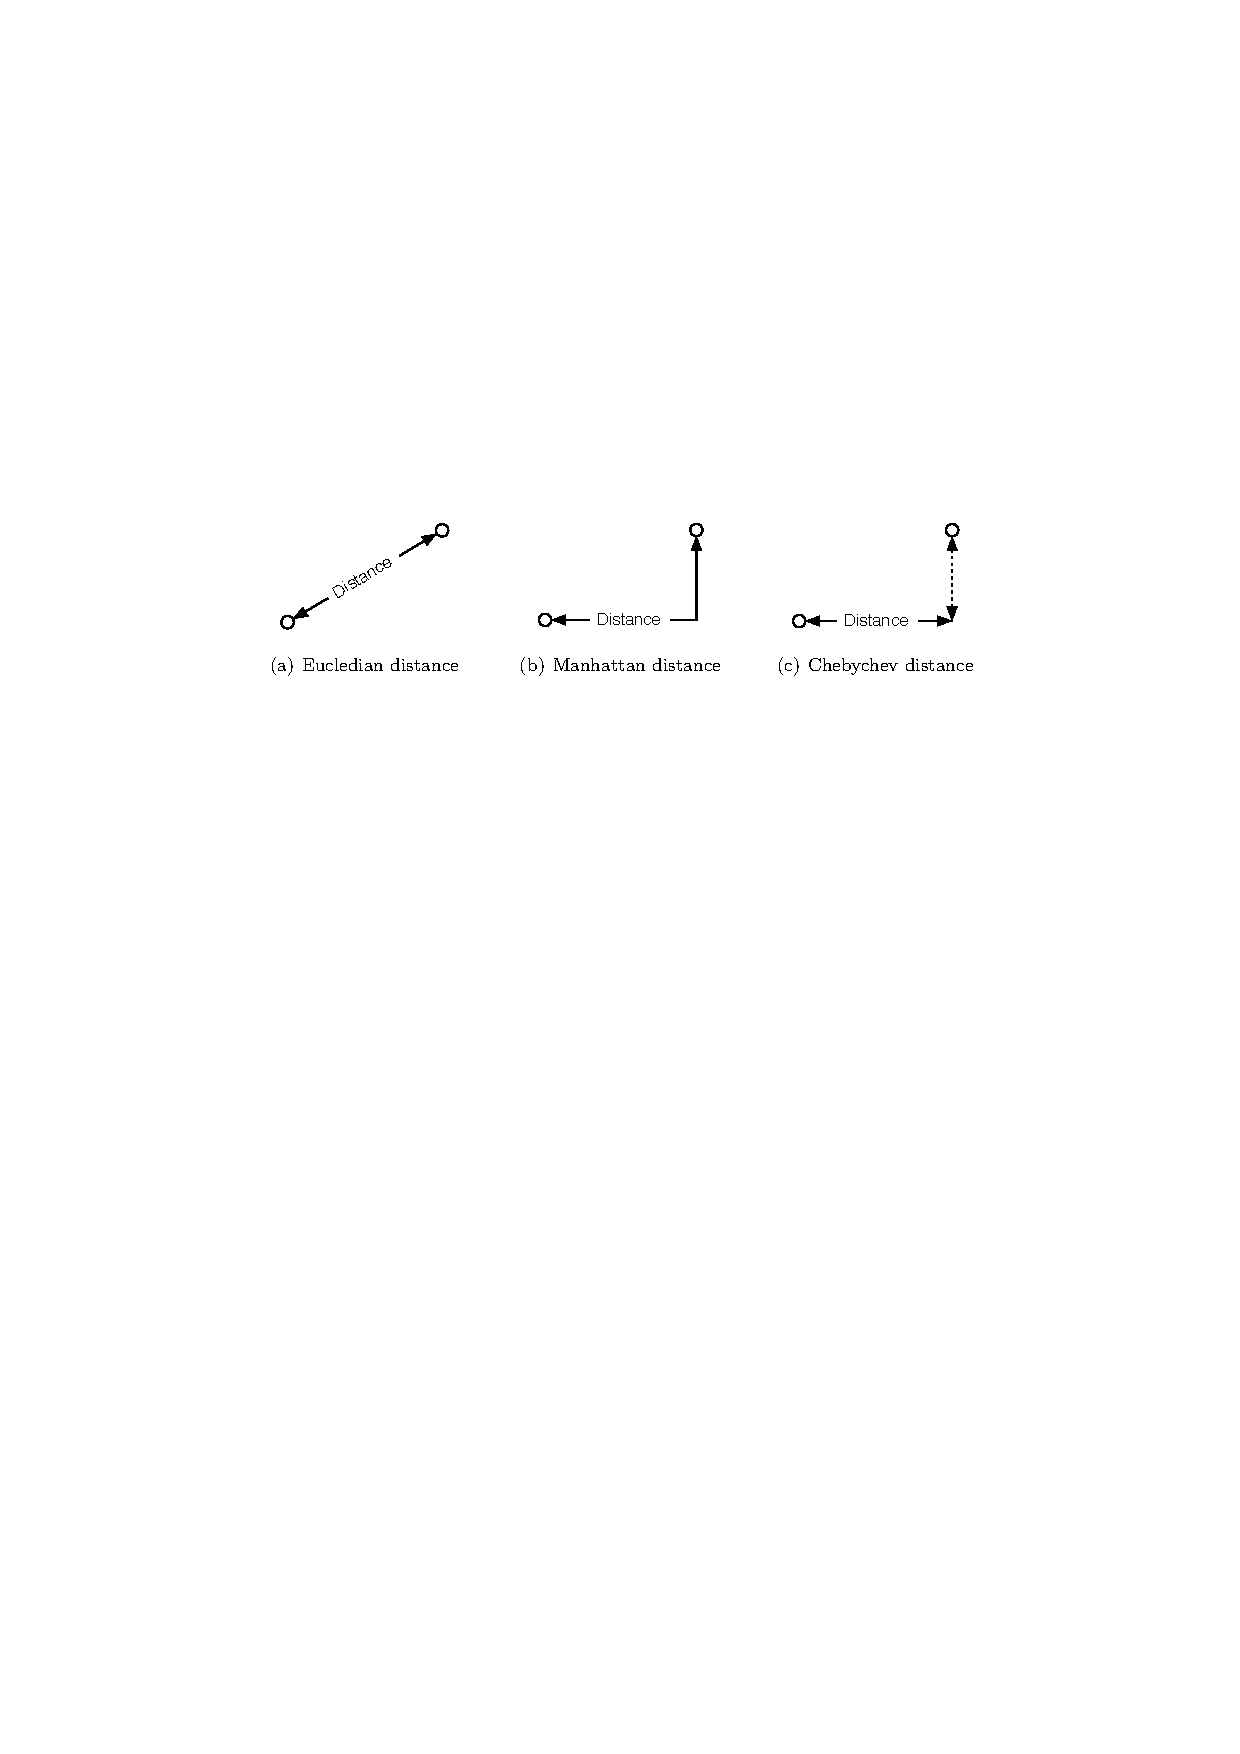
\includegraphics[width=1\textwidth]{figures/clustering_proximity.pdf}
    \caption{Distance measures for continuous data~\cite[p 12]{Meert06clustermaps}.}
    \label{fig:clustering-proximity}
  \end{center}
\end{figure}

\begin{itemize}

\item \textbf{Euclidian distance}. The euclidian distance is the geometric distance in the n-dimensional space. It is is the most common type of distance and defined as
\[ distance(x, y) = \sqrt{\sum_{i} (x_i - y_i)^2} \]

\item \textbf{Manhattan distance}. The manhattan distance, also known as city-block distance is distance when walking from one point to another following the axes. Compare with walking by following a raster like in manhattan. It is defined as
\[ distance(x, y) = \sum_{i} |x_i - y_i| \]

\item \textbf{Chebychev distance}. This distance measure returns the maximum distance between two points on any dimensions. It may be appropriate where two items are defined as `different', if they are different on any one of the dimensions.
\[ distance(x, y) = max |x_i - y_i| \]

\end{itemize}

\subsection{Clustering algorithms}

Researchers have created a multitude of algorithms, each appropriate for a certain task. As we will find out later, the requirements to the spatial clustering algorithm for this thesis are specific, which out-rules most scientific clustering algorithms which are geared towards image recognition or other disciplines. To provide an overview and to understand the basic differentiation of clustering techniques explained in \ref{chapter:clustering-techniques}, in this chapter we will introduce 3 foundational clustering algorithms: \textit{K-means}, \textit{Agglomerative Hierarchical Clustering Algorithm} and \textit{DBSCAN}.

\begin{itemize}

\item \textbf{Squared Error Algorithms: K-means}. The K-means is the most commonly used and simple algorithm based on a \textit{squared error criterion}. It creates a one-level partitioning of the data items by dividing them into \textit{K} clusters. By starting with a random initial partition it iteratively reassigns the patterns to clusters based on similarity.  The clustering process is completed when a convergence criterion is met, i.e. no further reassignments happen. Clusters are defined by \textit{cluster prototypes}: the centroid of the clustered items. Alternatively, the \textit{K-medoid} algorithm uses the most representative data item instead of the centroid.

The time complexity of the K-means algorithm is linear to the number of points:
\[time~complexity = \BigO{n}\]

\begin{algorithm}[t]
  \SetKwInOut{Input}{input}
  \Input{the number of clusters, $K$}
  \BlankLine
  {Select $K$ points as initial centroids}\;
  \While{Centroids do change}{
    {Form $K$ clusters by assigning each point to its closest centroid}\;
    {Recompute the centroid of each cluster}\;
  }
  \caption{K-means algorithm~\cite{Meert06clustermaps}}
  \label{alg:k-means}
\end{algorithm}

The selection of initial centroids affects the final outcome of the clustering process. Choosing them randomly is a simple but not very affective approach which can be compensating by applying multiple runs of the algorithm to retrieve an optimal result set. Optimizations to the centroid initialization include applying a hierarchical clustering or choosing distant points in the beginning.

Assigning points to the closest centroid requires a proximity measure, as explained in \ref{chapter:proximity}. Simple measures like the Euclidian distance are preferred, as this step needs to happen repeatedly within the algorithm. For each cluster, the centroid needs to be recalculated afterwards. This procedure is repeated until centroids do not change any more \cite{Jain99clusterreview, Meert06clustermaps}.

Figure \ref{fig:clustering_k-means} illustrates a K-means clustering process.

\begin{figure}[h]
  \begin{center}
    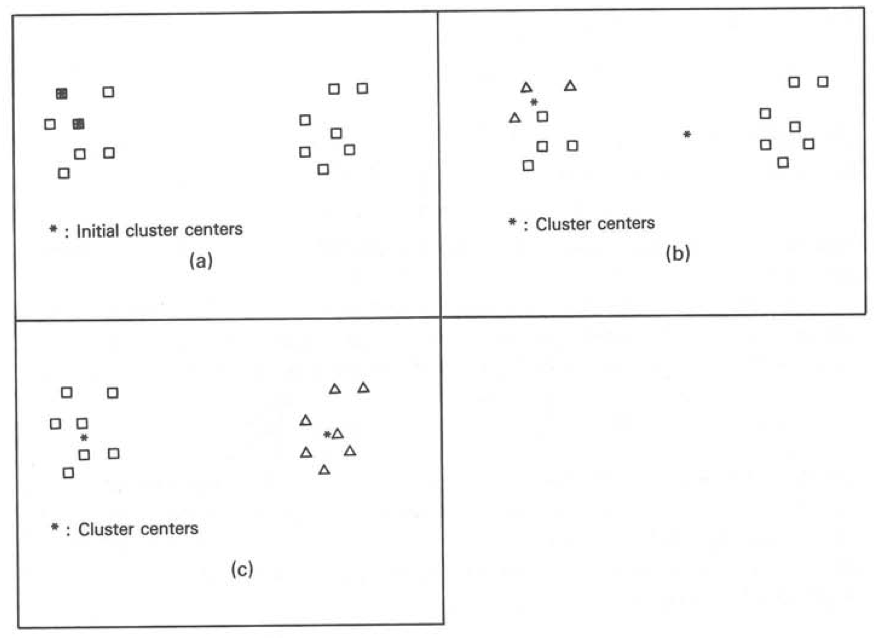
\includegraphics[width=0.9\textwidth]{figures/clustering_k-means.png}
    \caption{Convergence of K-means clustering: (a) initial data; (b) cluster membership after first loop; (c) cluster membership after second loop~\cite[p 99]{Jain88clustering}.}
    \label{fig:clustering_k-means}
  \end{center}
\end{figure}


\item \textbf{Agglomerative Hierarchical Clustering Algorithm}. This exemplary hierarchical clustering algorithm creates a hierarchy of nested sub clusters by serial partitioning. Its \textit{agglomerative} nature makes it start with every data item as a single clusters which get merged sub-sequentially. Alternatively, a \textit{divisive} hierarchical clustering would start with one cluster containing all data points and recursively split them up. At each level, a partitioning can be extracted, for example to serve as initial set of centroids for the previously discussed K-means algorithm. 

The time complexity of the agglomerative hierarchical clustering algorithm is:
\[time~complexity = \BigO{n^3}\]

\begin{algorithm}[t]
  {Assign each point to its individual cluster}\;
  {Compute the proximity matrix}\;
  \While{Number of clusters is larger than one}{
    {Merge the closest two clusters}\;
    {Update the proximity matrix to reflect the proximity between the new cluster and the original clusters}\;
  }
  \caption{Agglomerative hierarchic algorithm~\cite{Meert06clustermaps}}
  \label{alg:hierarchical}
\end{algorithm}

At the beginning of the agglomerative hierarchical clustering algorithm, each point is assigned to its own cluster. A proximity matrix is calculated that stores the distance of each pair of data item based on the chosen proximity measure.

To merge the two closest clusters, different heuristics may be applied. Most importantly, \textit{single-link} hierarchical clustering algorithms measure the distance between two clusters by the \textit{minimum} distance between all pairs of items from the two clusters. In contrast, \textit{complete-link} algorithms use the \textit{maximum} distance to create compact clusters and prevent chaining effects. Other approaches are based on \textit{average linkage} or \textit{Ward's method}. After merging the clusters, the proximity matrix will be updated so it reflects the current state of the clustering process. This procedure is repeated until all clusters have been merged, each step in the loop yields a level in the hierarchical clustering~\cite{Jain88clustering, Jain99clusterreview, Meert06clustermaps}.

Figure~\ref{fig:clustering-hierarchical-dendrogram} illustrates a Agglomerative Hierarchical clustering process as a dendrogram.

\begin{figure}[h]
  \begin{center}
    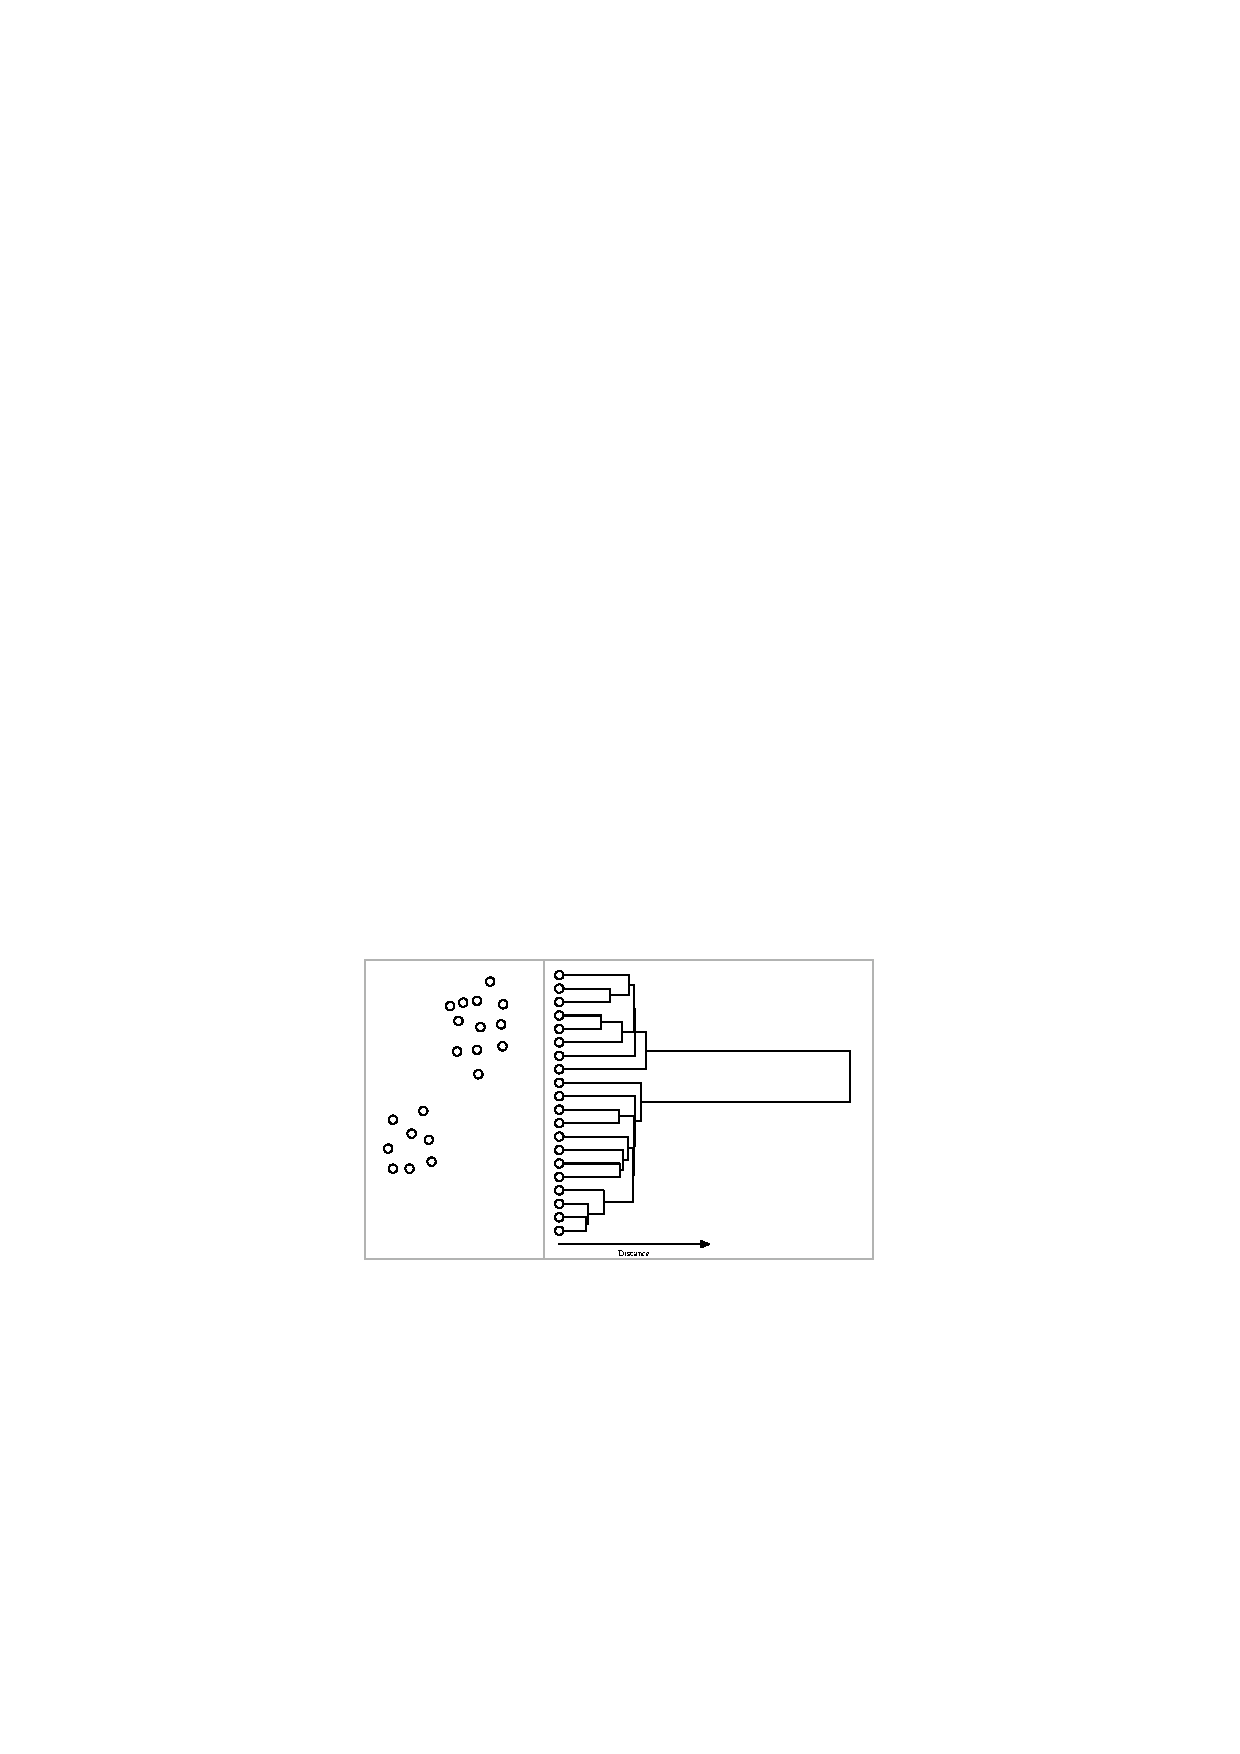
\includegraphics[width=0.9\textwidth]{figures/clustering_hierarchical_dendrogram.pdf}
    \caption{Dendrogram~\cite[p 20]{Meert06clustermaps}.}
    \label{fig:clustering-hierarchical-dendrogram}
  \end{center}
\end{figure}


\item \textbf{Density-based clustering algorithms: DBSCAN}. Density-based algorithms cluster regions of high density and separate them from regions with lower density. The density-based approach differentiates them from the previously discussed distance-based methods. This helps them overcome limitations of the former, as those tend to perform well in the detection of spherical-shaped clusters but perform weaker at discovering arbitrary shapes. Density-based algorithms are also insensitive to noise points, so that outliers get isolated. DBSCAN takes a center-based approach.
?
\begin{algorithm}[t]
  \While{Point is unclassified}{
    {Find points within region $\epsilon$}\;
    \If{number of points within region $> MinPts$} {
      {Start new cluster with Point}\;
      {Search regions of points in new cluster and expand cluster}\;
    }
  }
  \caption{DBSCAN algorithm~\cite{Meert06clustermaps}}
  \label{alg:dbscan}
\end{algorithm}

\textit{DBSCAN} starts with an unclassified point. Density is calculated by computing all points within a radius $\epsilon$. Based on the density, it classifies points as \textit{core points} if the number of points within neighborhood exceeds a threshold defined as $MinPts$. \textit{Border points} don't match the previous criterion but fall into the neighborhood of a core point. Finally \textit{noise points} are outside of any neighborhood and therefore are neither core points nor border points. Any core point will be expanded to a cluster in the procedure until every point has been classified~\cite{Varlaro08spatial, Meert06clustermaps}.

The quadratic time complexity of DBSCAN \BigO{n^2} can be optimized by using an indexing structure for the neighborhood queries~\cite{wiki:DBSCAN}:
\[time~complexity = \BigO{n \log{n} }\]



Figure~\ref{fig:clustering-dbscan} illustrates a DBSCAN clustering process.

\begin{figure}[h]
  \begin{center}
    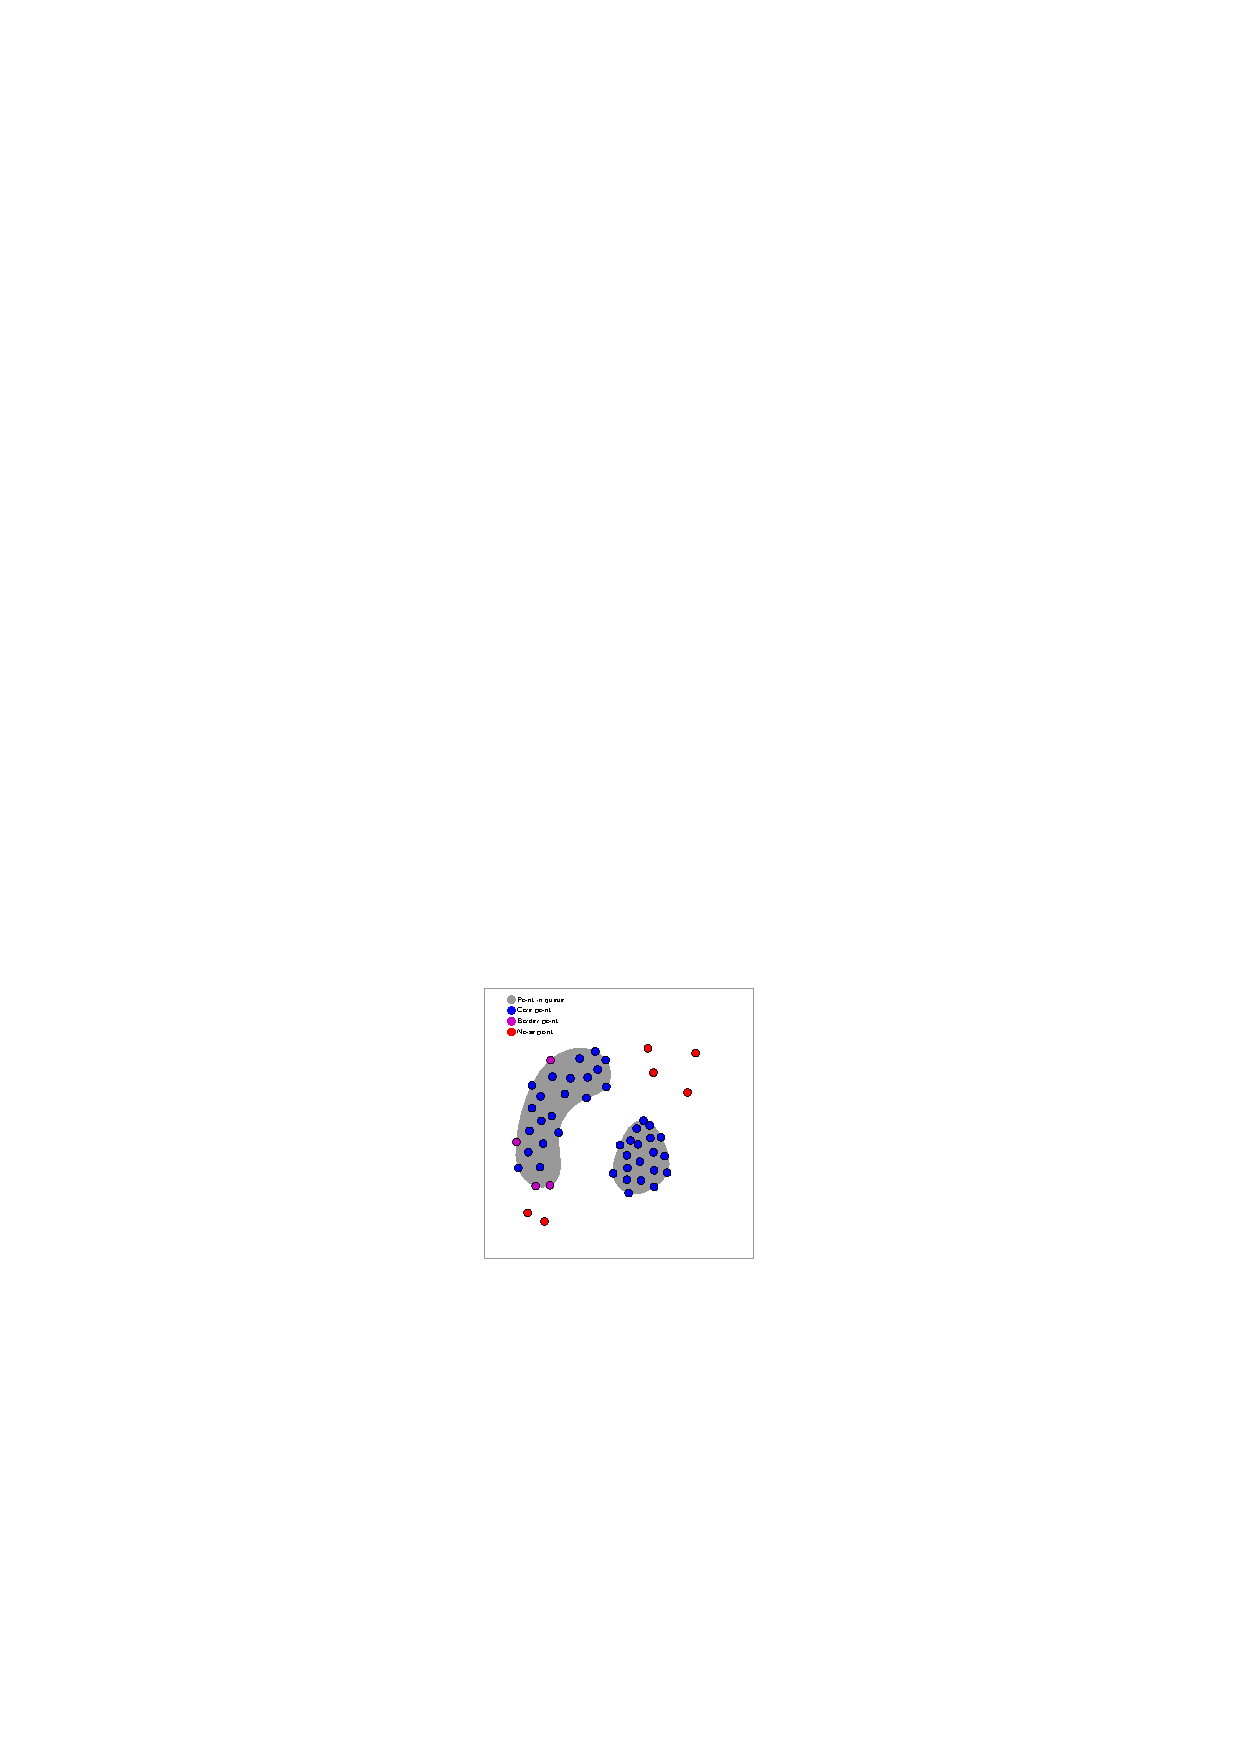
\includegraphics[width=0.55\textwidth]{figures/clustering_dbscan.pdf}
    \caption{DBSCAN algorithm~\cite[p 26]{Meert06clustermaps}.}
    \label{fig:clustering-dbscan}
  \end{center}
\end{figure}

\item \textbf{Grid-based algorithms: STING}. 

\end{itemize}





























%
% foundations - clustering algorithms
%

\section{Clustering algorithms}

Researchers have created a multitude of algorithms, each appropriate for a certain task. As we will find out later, the requirements to the spatial clustering algorithm for this thesis are specific, which out-rules most scientific clustering algorithms which are geared towards image recognition or other disciplines. To provide an overview and to understand the basic differentiation of clustering techniques explained in \ref{chapter:clustering-techniques}, in this chapter we will introduce 4 foundational clustering algorithms:

\begin{itemize}
\item {K-means (Squared Error Algorithm)}
\item {Agglomerative Hierarchical Clustering Algorithm}
\item {DBSCAN (Density-based)}
\item {STING (Grid-based)}
\end{itemize}

\subsection{Squared Error Algorithms: K-means}
\label{chapter:k-means}

The K-means is the most commonly used and simple algorithm based on a \textit{squared error criterion}. It creates a one-level partitioning of the data items by dividing them into \textit{K} clusters. By starting with a random initial partition, it iteratively reassigns the patterns to clusters based on similarity.  The clustering process is completed when a convergence criterion is met, i.e. no further reassignments happen. Clusters are defined by \textit{cluster prototypes}: the centroid of the clustered items. Alternatively, the \textit{K-medoid} algorithm uses the most representative data item instead of the centroid.

The time complexity of the K-means algorithm is linear to the number of points:
\[time~complexity = \BigO{n}\]

\begin{algorithm}[t]
  \SetKwInOut{Input}{input}
  \Input{the number of clusters, $K$}
  \BlankLine
  {Select $K$ points as initial centroids}\;
  \While{Centroids do change}{
    {Form $K$ clusters by assigning each point to its closest centroid}\;
    {Recompute the centroid of each cluster}\;
  }
  \caption{K-means algorithm~\cite{Meert06clustermaps}}
  \label{alg:k-means}
\end{algorithm}

The selection of initial centroids affects the final outcome of the clustering process. Choosing them randomly is a simple, but not very affective approach. This can be compensated by applying multiple runs of the algorithm, to retrieve an optimal result set. Optimizations to the centroid initialization include applying a hierarchical clustering or selecting distant points in the beginning.

Assigning points to the closest centroid requires a proximity measure, as explained in \ref{chapter:proximity}. Simple measures like the Euclidian distance are preferred, as this step needs to happen repeatedly within the algorithm. For each cluster, the centroid needs to be recalculated afterwards. This procedure is repeated until centroids do not change any more \cite{Jain99clusterreview, Meert06clustermaps}.

Figure \ref{fig:clustering_k-means} illustrates a K-means clustering process.

\begin{figure}[h]
  \begin{center}
    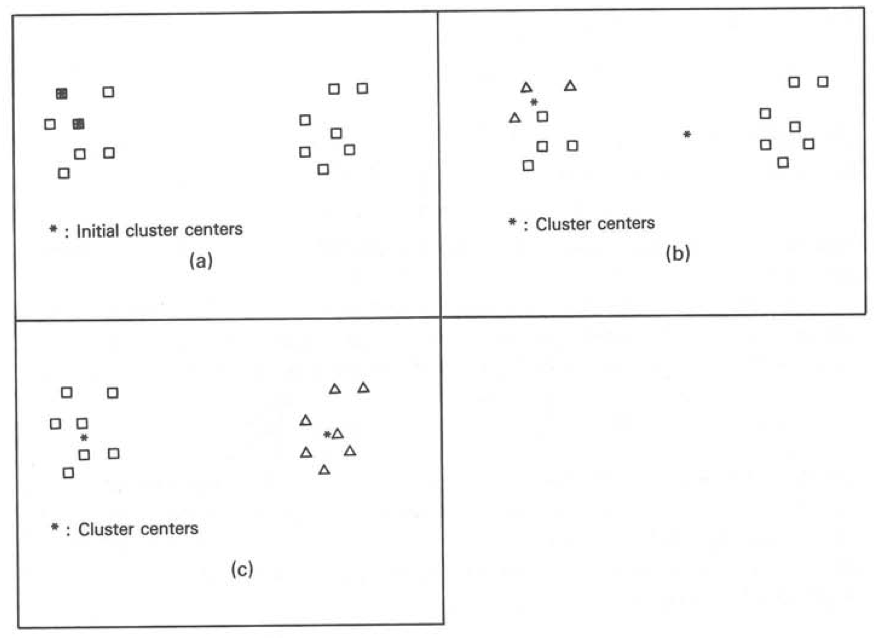
\includegraphics[width=1\textwidth]{figures/clustering_k-means.png}
    \caption{Convergence of K-means clustering: (a) initial data; (b) cluster membership after first loop; (c) cluster membership after second loop~\cite[p 99]{Jain88clustering}.}
    \label{fig:clustering_k-means}
  \end{center}
\end{figure}


\subsection{Agglomerative Hierarchical Clustering Algorithm}
\label{chapter:clustering-hierarchical}

This exemplary, \textit{hierarchical clustering algorithm} creates a hierarchy of nested sub clusters by serial partitioning. Its \textit{agglomerative} nature makes it start with every data item as a single cluster and merge them sub-sequentially. As an alternative, a \textit{divisive} hierarchical clustering would start with one cluster containing all data points and recursively split them up. At each level, a partitioning can be extracted, for example to serve as initial set of centroids for the previously discussed K-means algorithm. 

The time complexity of the agglomerative hierarchical clustering algorithm is:
\[time~complexity = \BigO{n^3}\]

\begin{algorithm}[t]
  {Assign each point to its individual cluster}\;
  {Compute the proximity matrix}\;
  \While{Number of clusters is larger than one}{
    {Merge the closest two clusters}\;
    {Update the proximity matrix to reflect the proximity between the new cluster and the original clusters}\;
  }
  \caption{Agglomerative hierarchic algorithm~\cite{Meert06clustermaps}}
  \label{alg:hierarchical}
\end{algorithm}

At the beginning of the agglomerative hierarchical clustering algorithm, each point is assigned to its own cluster. A proximity matrix is calculated to store the distances for all pairs of data items based on the chosen proximity measure.

To merge the two closest clusters, different heuristics may be applied. Most importantly, \textit{single-link} hierarchical clustering algorithms measure the distance between two clusters by the \textit{minimum} distance between all pairs of items from the two clusters. In contrast, \textit{complete-link} algorithms use the \textit{maximum} distance to create compact clusters and prevent chaining effects. Other approaches are based on \textit{average linkage} or \textit{Ward's method}. After merging the clusters, the proximity matrix will be updated, so that it reflects the current state of the clustering process. This procedure is repeated until all clusters have been merged, each step in the loop yields a level in the hierarchical clustering~\cite{Jain88clustering, Jain99clusterreview, Meert06clustermaps}.

Figure~\ref{fig:clustering-hierarchical-dendrogram} illustrates a Agglomerative Hierarchical clustering process as a dendrogram.

\begin{figure}[h]
  \begin{center}
    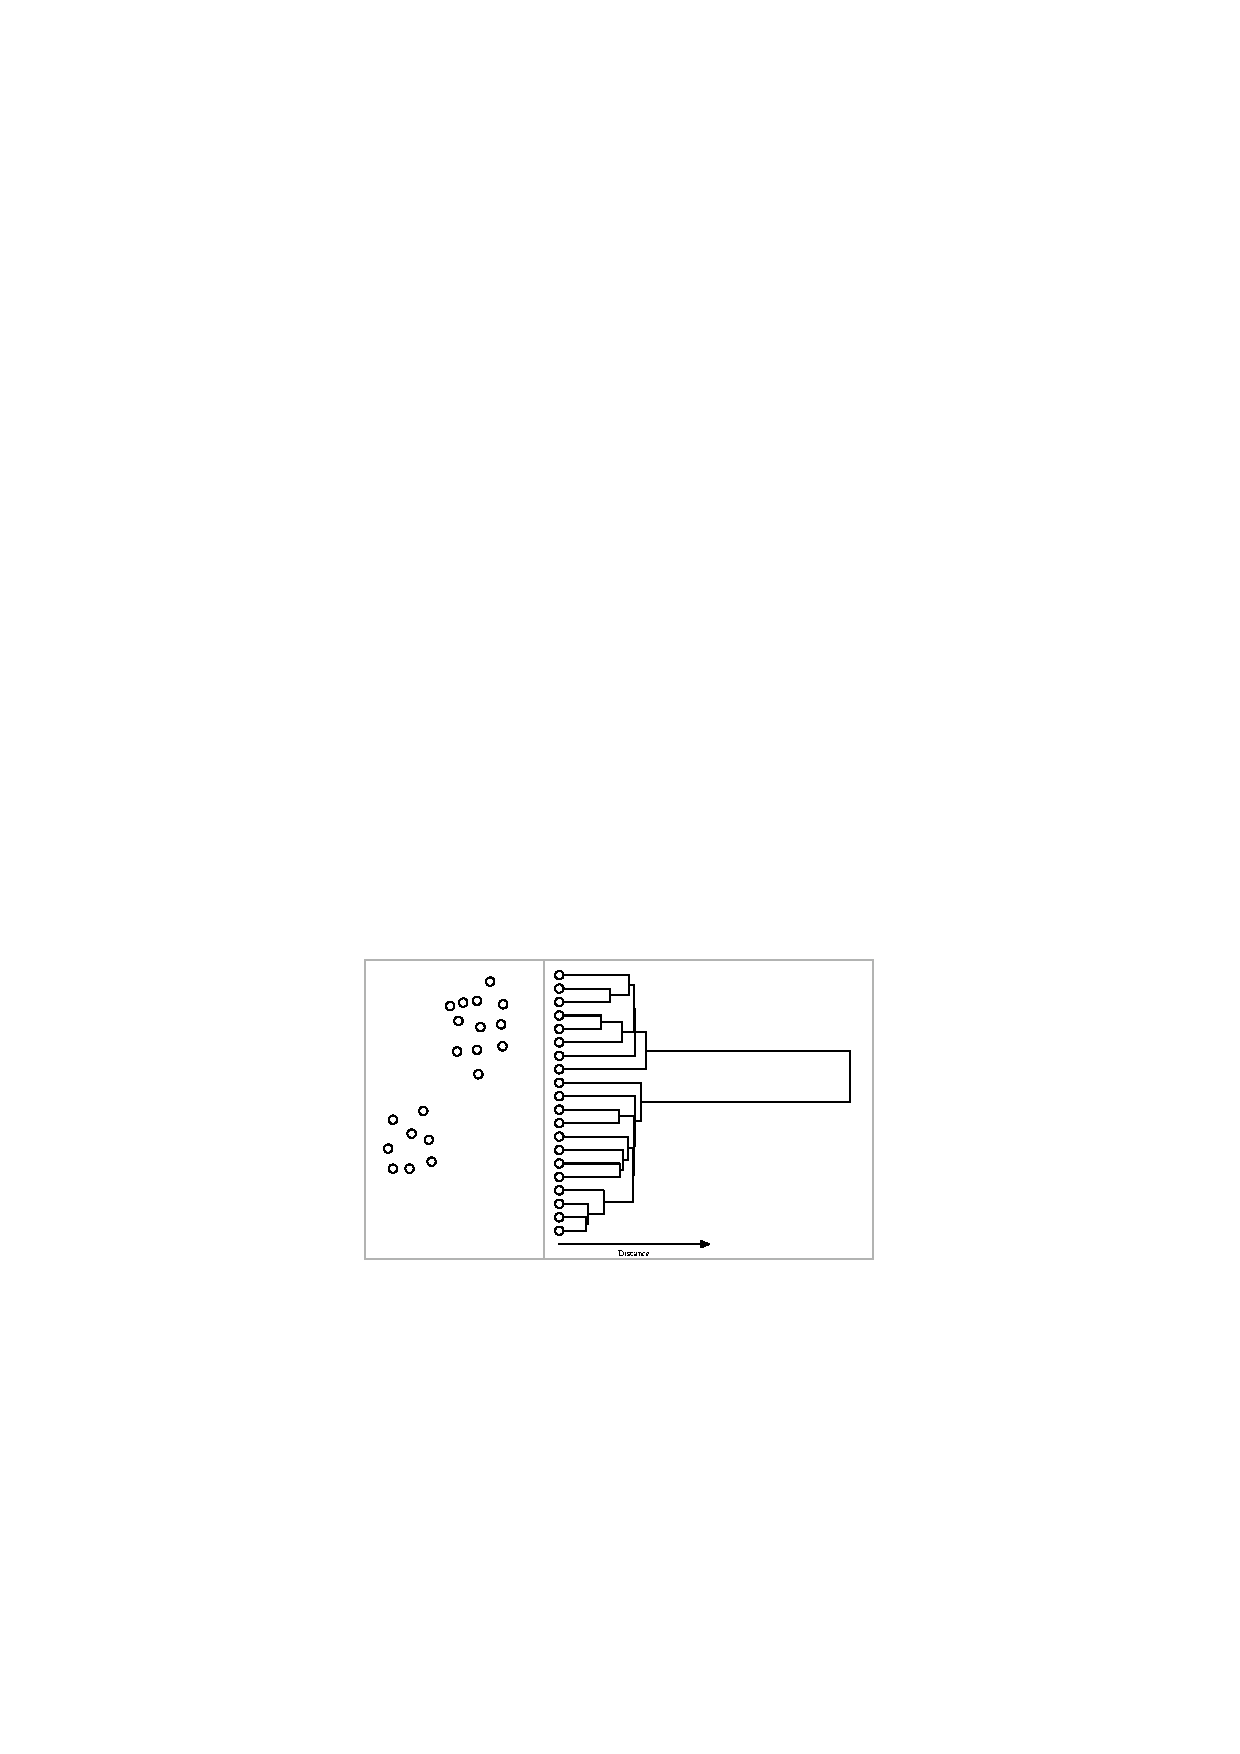
\includegraphics[width=0.9\textwidth]{figures/clustering_hierarchical_dendrogram.pdf}
    \caption{Dendrogram~\cite[p 20]{Meert06clustermaps}.}
    \label{fig:clustering-hierarchical-dendrogram}
  \end{center}
\end{figure}


\subsection{Density-based clustering algorithms: DBSCAN}

Density-based algorithms cluster regions of high density and separate them from regions with lower density. The density-based approach is different to the previously discussed distance-based methods. Those tend to perform well in the detection of spherical-shaped clusters, but discovering arbitrary shapes is a problem. Density-based algorithms overcome this limitation and are also insensitive to noise points, so that outliers get isolated.

\begin{algorithm}[t]
  \While{Point is unclassified}{
    {Find points within region $\epsilon$}\;
    \If{number of points within region $> MinPts$} {
      {Start new cluster with Point}\;
      {Search regions of points in new cluster and expand cluster}\;
    }
  }
  \caption{DBSCAN algorithm~\cite{Meert06clustermaps}}
  \label{alg:dbscan}
\end{algorithm}

\textit{DBSCAN} starts with an unclassified point. Subsequently, the density of the point is calculated by computing all its neighborhood points within a radius $\epsilon$. Based on the density, the algorithm classifies points as \textit{core points}, \textit{border points} or \textit{noise points}:

\begin{itemize}
\item \textit{core points} have a number of points within their neighborhood that exceeds the threshold defined as $MinPts$
\item \textit{border points} don't match the previous criterion but they themselves fall into the neighborhood of another core point
\item \textit{noise points} are outside of any neighborhood and therefore are neither core points nor border points
\end{itemize}

Any core point will be expanded to a cluster in the procedure until every point has been classified~\cite{Varlaro08spatial, Meert06clustermaps}.

The quadratic time complexity of DBSCAN \BigO{n^2} can be optimized by using an indexing structure for the neighborhood queries~\cite{wiki:DBSCAN}:
\[time~complexity = \BigO{n \log{n} }\]

Figure~\ref{fig:clustering-dbscan} illustrates a DBSCAN clustering process.

\begin{figure}[h]
  \begin{center}
    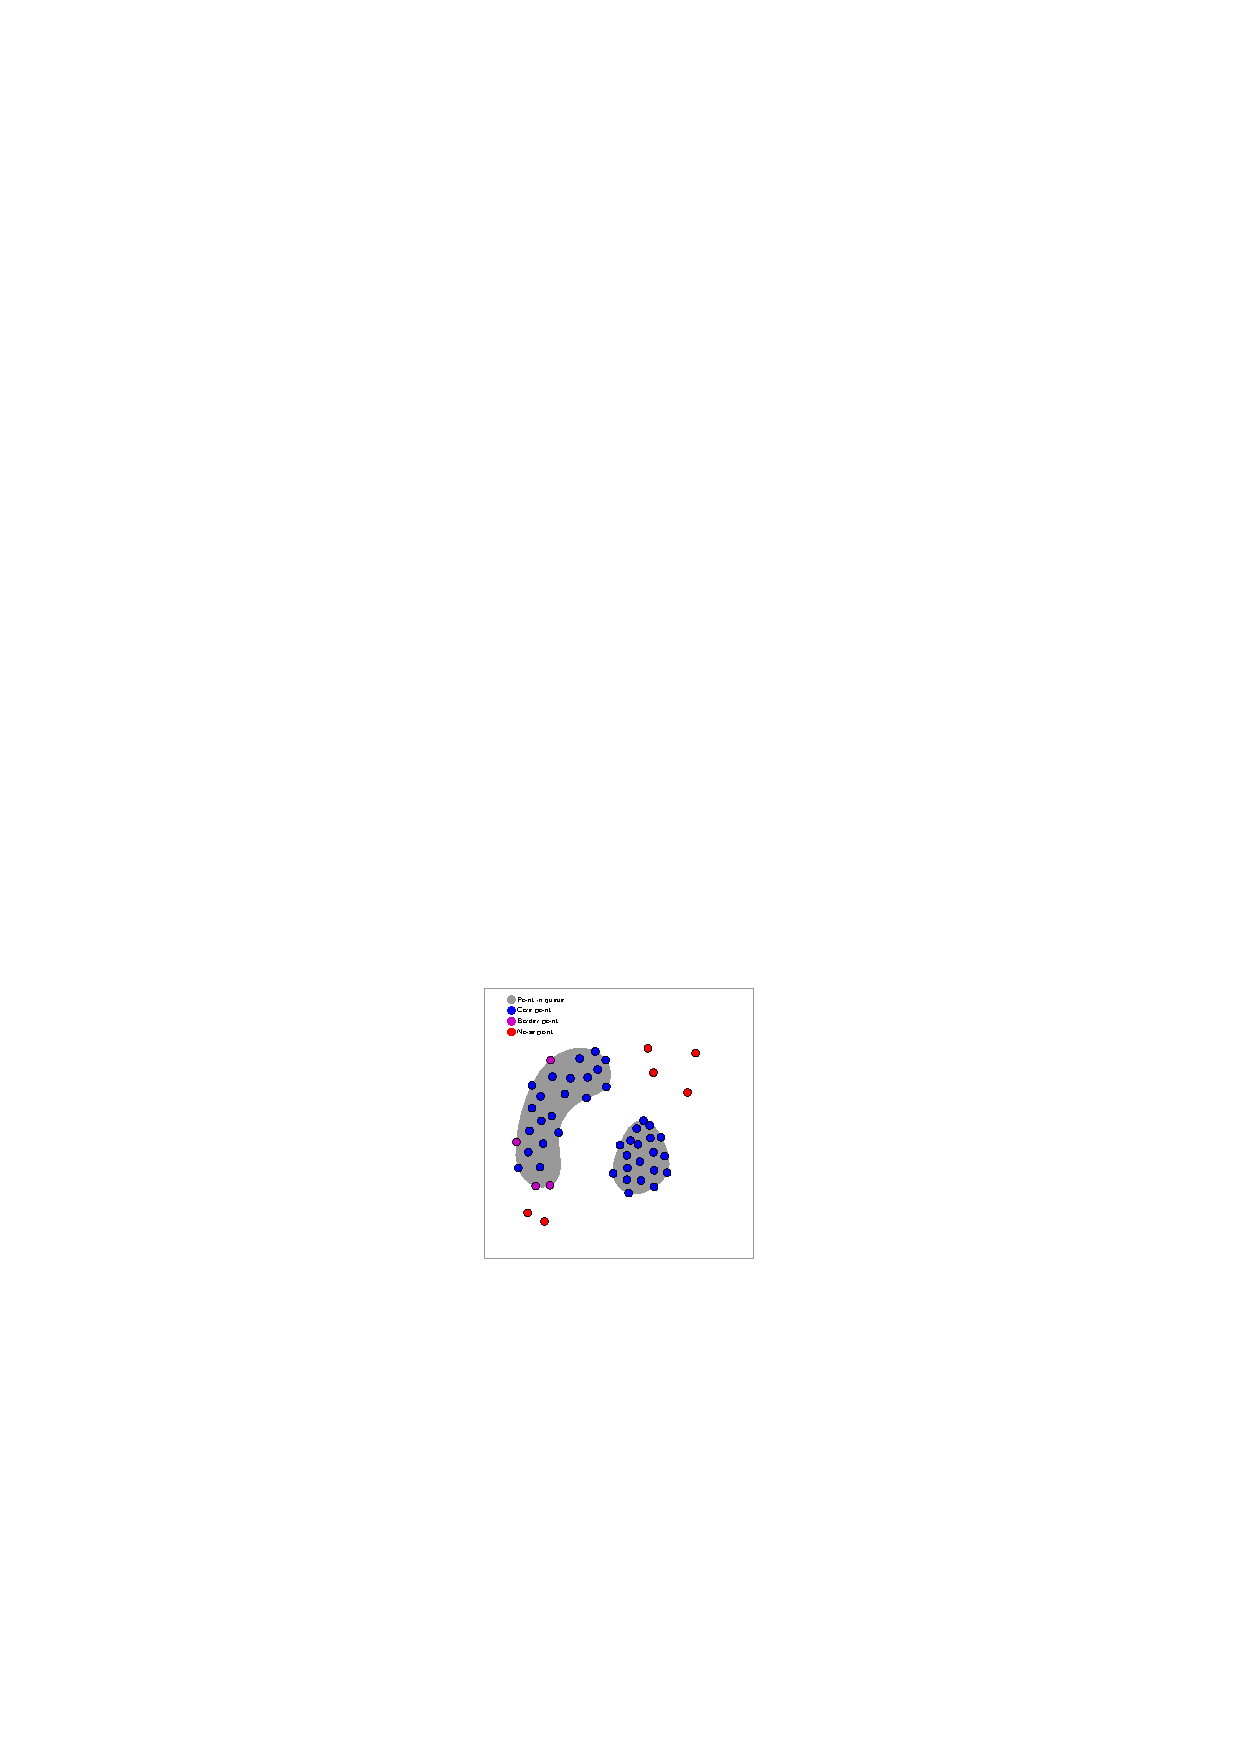
\includegraphics[width=0.55\textwidth]{figures/clustering_dbscan.pdf}
    \caption{DBSCAN algorithm~\cite[p 26]{Meert06clustermaps}.}
    \label{fig:clustering-dbscan}
  \end{center}
\end{figure}

\subsection{Grid-based algorithms: STING}
\label{chapter:clustering-grid}

The time complexity of the previously discussed algorithms is at least linear to the number of points that have to be clustered. Grid-based algorithms overcome this performance limitation by partitioning data to be clustered in a grid structure. The clustering process is executed on pre clustered cells of the grid structure, which obviously scales better.

The STING algorithm takes such a grid-based approach and divides the data points into a grid of rectangular cells. The cells form a hierarchical structure, so that different levels of grids correspond to different resolutions. Every cell in the grid is sub-divided into a further partitioning one level deeper in the hierarchy. STING therefore precomputes a hierarchical index with various levels of granularity on which the clustering process is later executed. The name-giving property of STING (Statistical INformation Grid) is that each cell contains statistical information which can be used to answer queries. 

The time complexity can be shifted to the computation of the grid which is linear to the points of data $\BigO{n}$. The query processing time is reduced to $\BigO{g}$, where $g$ is the constant of number of cells at the bottom level of the computed hierarchy. As per the construction of the hierarchy, it can be assumed that $g \ll n$~\cite{Varlaro08spatial, Wang97sting}.  

Figure~\ref{fig:clustering-sting} illustrates a hierarchical grid used in the STING clustering process.

\begin{figure}[h]
  \begin{center}
    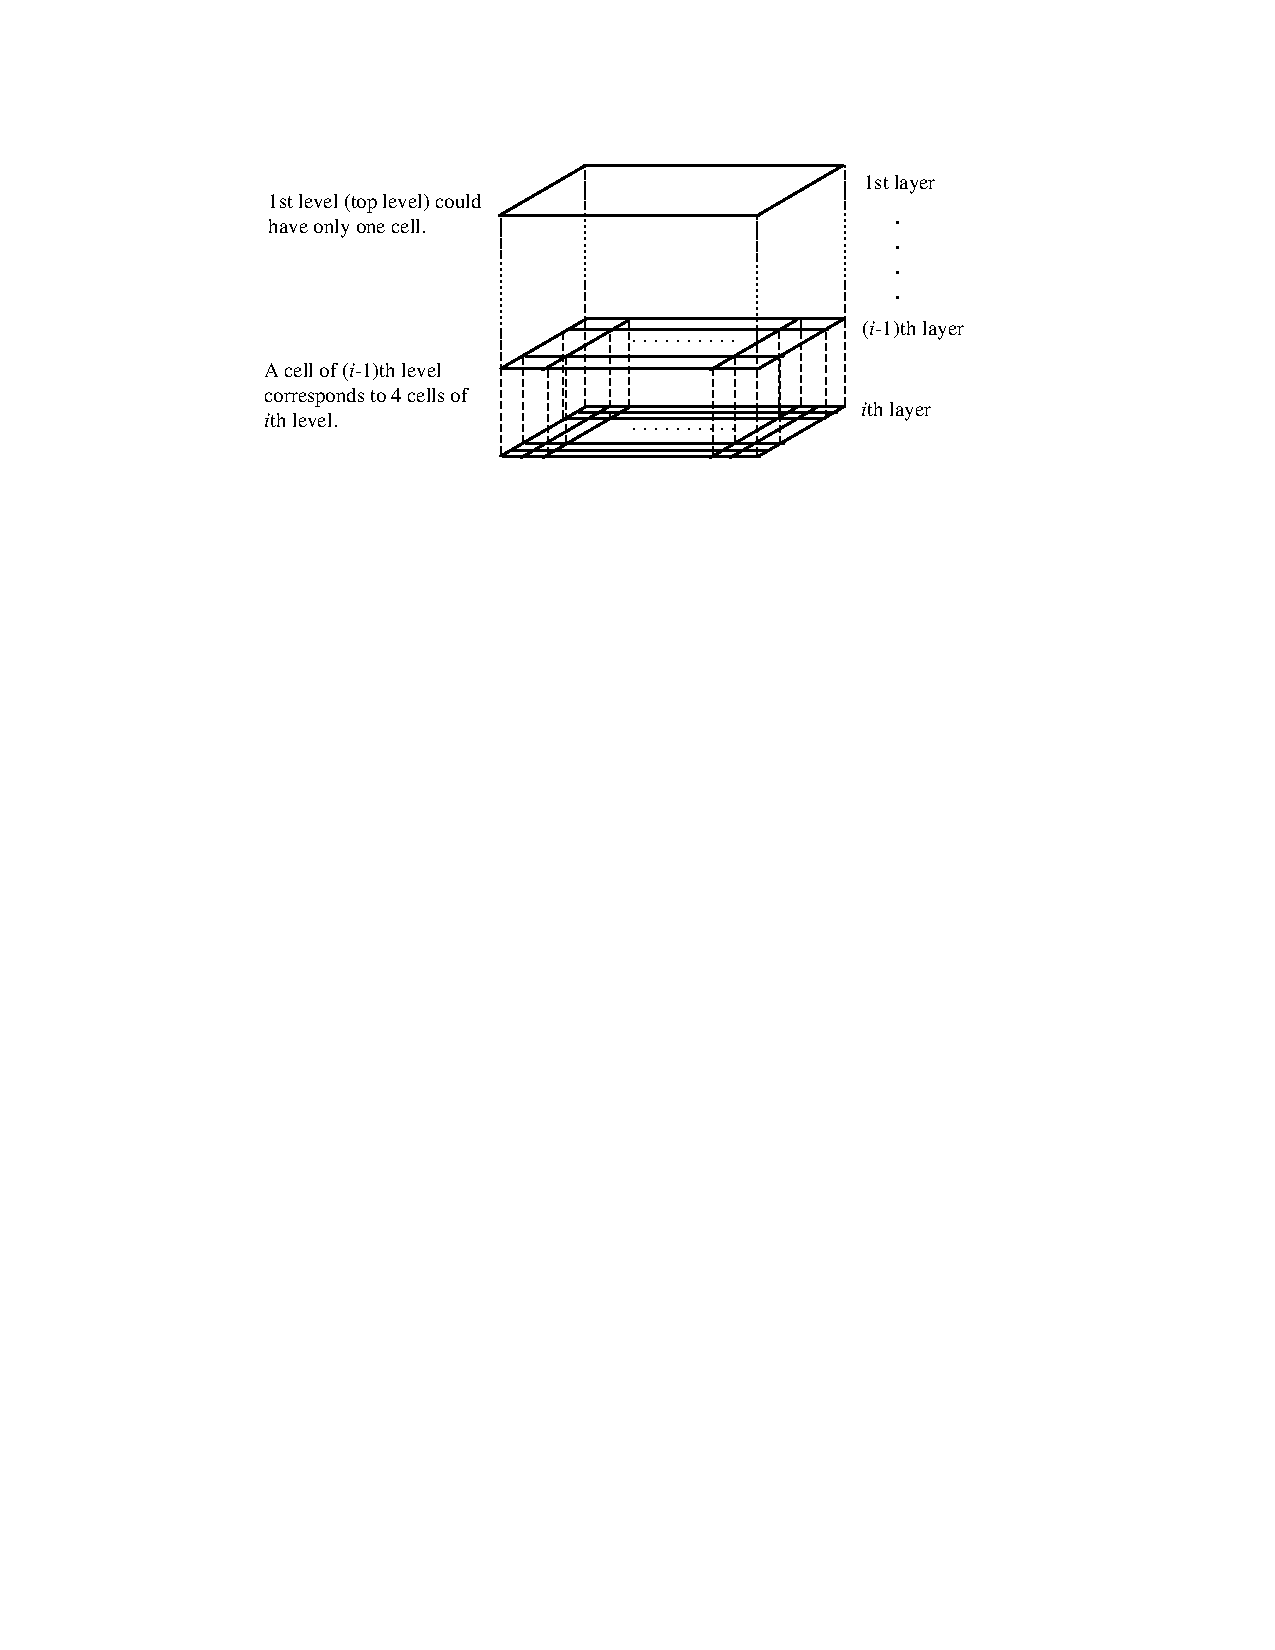
\includegraphics[width=0.9\textwidth]{figures/clustering_sting.pdf}
    \caption{Hierarchical Structure of the STING algorithm~\cite[p 5]{Wang97sting}.}
    \label{fig:clustering-sting}
  \end{center}
\end{figure}























%
% foundations - spatial data
%

\section{Spatial data}
\label{chapter:spatial-data}

A central aspect in web mapping is dealing with spatial data. Decisions on how to structure and store spatial data highly influence the computation tasks that may be performed on such data. This mainly depends on the type of spatial data, where points are the most basic of all. Depending on the use case, different types of data are to be represented and stored: points, lines, rectangles, regions, surfaces and/or volumes. While most of the discussed concepts may be extended or generalized for processing more complex types of data, this is out of scope for this thesis. Instead, we focus on points as the most common type of spatial data~\cite{Samet90spatialdata}.

One fundamental way to store spatial data is the quadtree, a hierarchical data structure based on recursive decomposition of space. Hanan Samet attributes the history of quadtrees (and octrees which are their 3-dimensional extension) to Dijkstra, who invented a one-level decomposition of a matrix into square blocks. Morton then applied this technique to creating a spatial index (z-order). We will first discuss space orders \& decomposition and then put those into context when outlining the basics of the quadtree.


\subsection{Space order methods}
\label{chapter:space-order}

In order to store multi-dimensional, spatial data in a sequential storage like computer memory, the data needs to be serialized. Consider a pixel image as an example. Its 2-dimensional pixel values are positioned in planar space. In order to store the image, those pixels have to be processed in a predefined order, such that they can be serialized into a 1-dimensional array of memory units.

The traditional order for storing a raster of image data was row by row. The row order sequentially processes the raster row by row from left to right, starting at the top left corner. In contrast, the row-prime order switches the horizontal processing direction at the end of each row. This leads to a higher locality as it has the property of always moving to a 4-neighbor~\cite{Goodchild83raster}.

Besides the discussed row orders, additional space-ordering methods have been developed to serve different purposes. The Morton and Peano-Hilbert orders both visit entire sub quadrants first before before exiting them. The Morton order is easier to compute, because the position (key) of each element in the ordering can be determined by interleaving the bits of the x and y coordinates of that element. One disadvantage of the Morton order are the gaps: the longest move in a raster of $2^n$ by $2^n$ is one column and $2^n - 1$ rows (or vice versa). A better locality is offered by the Hilbert-Peano order which always has the property of moving to a 4-neighbor. This advantage on the other hand has the cost of a more complex definition. Calculating keys for the Hilbert-Peano order is more difficult. The higher complexity of the Hilbert-Peano obviously shows that its recursion is harder to define as well. Figure~\ref{fig:space-orders} illustrates these fundamental space orders with two further ones that allow for ordering unbounded space in two (Cantor-diagonal order) or four directions (spiral order)~\cite{Samet90spatialdata}.

\begin{figure}[h]
  \begin{center}
    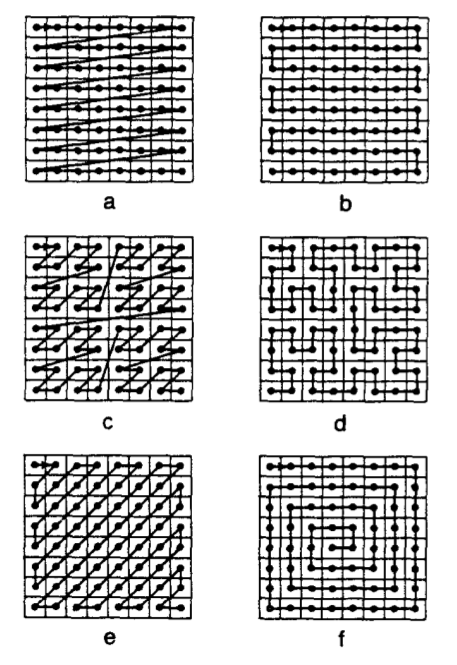
\includegraphics[width=0.5\textwidth]{figures/space_orders.png}
    \caption{The result of applying a number of different space-ordering methods to an $8 \times 8$ image whose first element is in the upper left corner of the image: (a) row order, (b) row-prime order, (c) Morton order, (d) Peano-Hilbert order, (e) Cantor-diagonal order, (f) spiral order~\cite[p 14]{Samet90spatialdata}.}
    \label{fig:space-orders}
  \end{center}
\end{figure}

The fact that the Hilbert-Peano order has the property of always moving to a 4-neighbor shouldn't be misinterpreted as still there are gaps. ``A bijective mapping from multidensional data to one dimension cannot be done the way that in any case nearby multidimensional points are also close together in one dimension~\cite{Tropf81multidimensional}''. Figure~\ref{fig:space-orders} clearly shows what Samet describes as ``both the Morton and Peano-Hilbert order exhaust a quadrant or subquadrant of a square image before exiting it~\cite{Samet90spatialdata}''. This means that the orders maintain locality for those quadrants based on the hierarchy, but the edges are still disconnected. The same issue will be dealt with further in Geohash (TODO Geohash).


\subsection{Space decomposition methods}

By definition, space decomposition methods partition space in a way so that,
\begin{itemize}
\item partitions are infinitely repetitive patterns for images of any size,
\item partitions are infinitely decomposable to generate finer sub-partitions of higher resolution.~\cite{Samet90spatialdata}
\end{itemize}

Various space decomposition methods exist. They can be classified depending on the shapes that are used for the partitioning patterns. Polygonal shapes are computationally simpler and can be used to approximate the interior of a region while non-polygonal shapes are more geared towards approximating the perimeter of region. Figure~\ref{fig:space-decomposition} visualizes a number of basic, polygon-based space decomposition methods. 

\begin{figure}[h]
  \begin{center}
    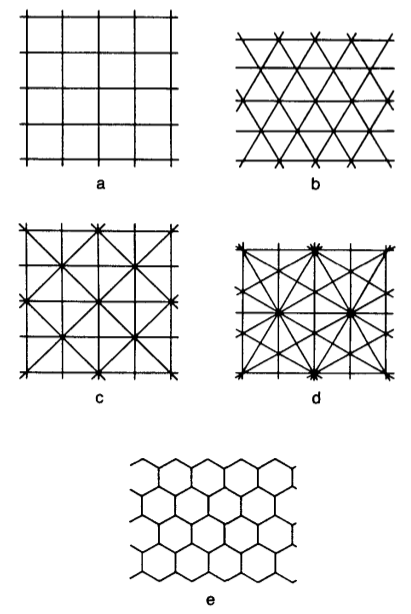
\includegraphics[width=0.5\textwidth]{figures/space_decompositions.png}
    \caption{Sample tessellations: (a) $[4^4]$ square; (b) $[6^3]$ equilateral triangle; (c) $[4.8^2]$ isoceles triangle; (d) $[4.6.12]$ 30-60 right triangle; (e) $[3^6]$ hexagon~\cite[p 17]{Samet90spatialdata}.}
    \label{fig:space-decompositions}
  \end{center}
\end{figure}

The simplest polygonal space decomposition method is based on squares. It is directly related to the Morton and Peano-Hilbert space order methods as described in the previous chapter \ref{chapter:space-order}. Both orders work in a hierarchical manner and visit entire sub-quadrants first before continuing further. This is why they are predestined to decomposing space into squares as indicated in Figures~\ref{fig:space-orders}~and~\ref{fig:space-decompositions}.

\subsection{Quadtree}

Quadtrees are hierarchical data structures based on recursive decomposition of space. Their original motivation was to optimize storage by aggregating identical or similar values. Over time they have also been studied to optimize execution time of spatial application and have been established as a common practice for representing and storing spatial data. The resolution of a quadtree can be fixed or variable and directly relates to the number of decomposition times of the space where the data points live. A standardized implementation is the region quadtree which subdivides space into four equal-sized quadrants.

\begin{figure}[h]
  \begin{center}
    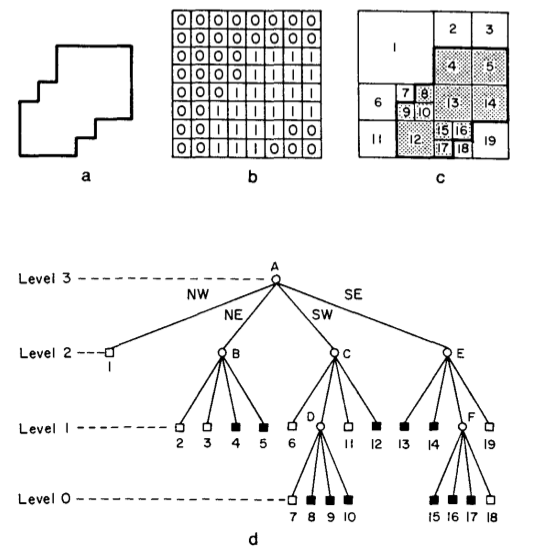
\includegraphics[width=0.7\textwidth]{figures/quadtree.png}
    \caption{An example of (a) a region, (b) its binary array, (c) its maximal blocks (blocks in the region are shaded), and (d) the corresponding quadtree~\cite[p 3]{Samet90spatialdata}.}
    \label{fig:space-decompositions}
  \end{center}
\end{figure}

Quadtrees can be constructed in different ways. A top-down approach implements the Morton order which maps the multidimensional data to one dimension and has been introduced in chapter~\ref{chapter:space-order}. Also note that the term quadtree has taken various meanings: actually it is a trie (or digital tree) structure because each data key is a sequence of characters. ``A node at depth $i$ in the trie represents an $M$-way branch depending on the $i$-th character'' \cite{Samet90spatialdata}.

\subsection{Geohash}
\label{chapter:geohash}

Geohash is a latitude/longitude geocode system based on the Morton order, described in \ref{chapter:space-order}. It encodes geographic point coordinates into string identifiers that reflect a hierarchical spatial structure. Its gradual precision degradation property means that if two geohashes share a common prefix, their closeness is described by the length of the shared prefix~\cite{wiki:geohash, Smiley11geohash}.

Originally, the geohash encoding algorithm has been developed and put into the public domain by Gustavo Niemeyer when creating the web service \href{http://geohash.org}{geohash.org}. The service allows to encode spatial coordinates into unique string identifiers and vice versa~\cite{wiki:geohash}. Amongst other applications, it has also been incorporated into geospatial search plugins of the Apache Solr search platform~\cite{Smiley11geohash} and leveraged for real-time, location-aware collaborative filtering of web content by HP Labs~\cite{Sand11geohashapp}.

A geohash is constructed by interleaving the bits of the latitude and longitude values and converting them into a string of characters using a Base 32 encoding. As every Base 32 symbol is represented by an uneven number of 5 bits, the resulting  space decomposition is a rectangular grid formed by $4 \times 8$ or $8 \times 4$ cells. The orientation of the resulting rectangles alternates between vertical for characters of an odd index and horizontal for such characters that are positioned at an even index within the geohash. Figure \ref{fig:geohash} illustrates how the first character of a geohash string splits the projected earth into an $8 \times 4$ grid of horizontally aligned rectangles~\cite{wiki:geohash, Smiley11geohash}.

\begin{figure}[h]
  \begin{center}
    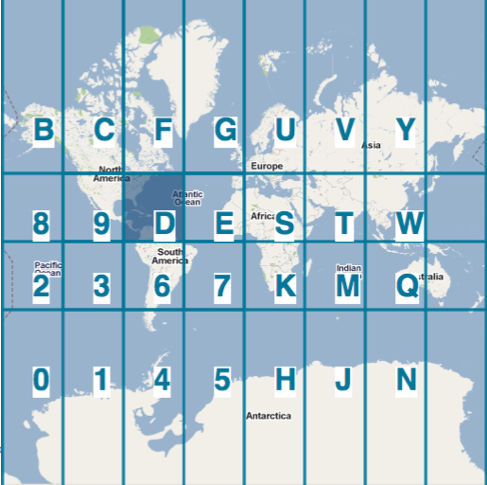
\includegraphics[width=0.7\textwidth]{figures/geohash_example.png}
    \caption{Space decomposition of the geohash algorithm on the first level~\cite{Smiley11geohash}.}
    \label{fig:geohash}
  \end{center}
\end{figure}

The fact that points with a common prefix are near each other must not be confused with the converse. Due to the nature of the morton order, edge cases exist. Two points may be very close to each other, without sharing an equally long prefix. Figure \ref{fig:geohash-edge} illustrates an example of two closely positioned points being located within different geohashes. The first point being at the very lower end of the ``DRT'' geohash and the second point positioned closely at the upper end of the ``DRM'' geohash. 

\begin{figure}[h]
  \begin{center}
    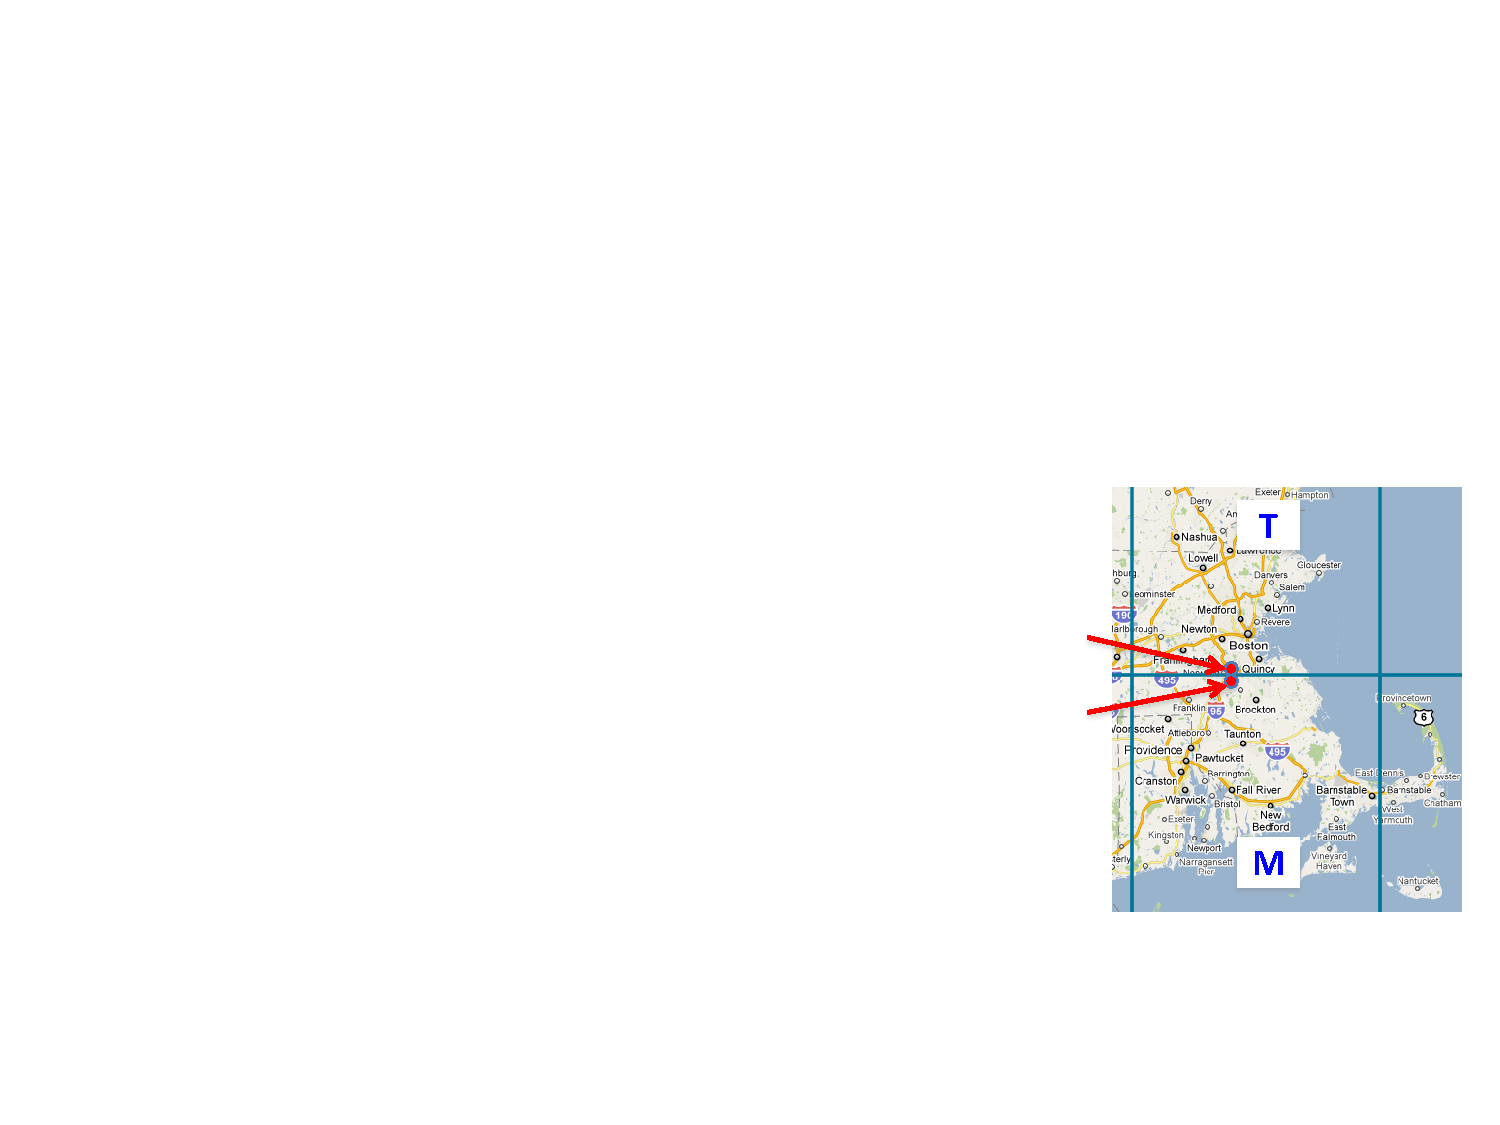
\includegraphics[width=0.7\textwidth]{figures/geohash_edges.pdf}
    \caption{Geohash edge case, where two closely positioned points do not share the same Geohash prefix~\cite{Smiley11geohash}.}
    \label{fig:geohash-edge}
  \end{center}
\end{figure}






























%
% foundations - mapping
%

\section{Web Mapping}

Maps have become an almost instinctive way of seeing our world. They probably first appeared over 18,000 years ago and already in the 16th century, they were produced in large numbers for navigational and military purposes. Maps are powerful tools that help organize boundaries and administrative activities. They allow telling stories, visualizing data and understanding geographic contexts
~\cite{Zzolo11mappingdrupal}.

Recently, Google Maps\footnote{\url{http://maps.google.com}} has made digital maps available to a large number of internet users. \textit{Digital natives} are used to navigate by using interactive maps on their smart phones and look up places on online maps on their computers.

Web mapping describes the whole process of designing, implementing, generating and delivering maps on the internet. It applies theoretical foundations from web cartography to the technical possibilities and boundaries of constantly evolving web technologies. The continuous development of related technologies has created a wide variety of \textit{types of web maps}: from analytic, animated, collaborative and dynamically created web maps to online atlases, realtime and static web maps~\cite{wiki:web-mapping}.

In order to represent spatial locations, \textit{reference systems} are used, that subdivide the geographic area into units of common shape and size. Such spatial reference systems consist of a \textit{coordinate system}, a \textit{datum} and a \textit{projection}. \textit{Geodetic datums} are models that approximate the shape of the Earth. In the following two chapters, the remaining concepts of coordinate systems and map projections will be explained in more detail.

\subsection{Coordinate systems}
\label{chapter:coordinates}

In mapping, a coordinate system is used to represent spatial locations in a numeric way. We mainly differentiate between \textit{Cartesian} and \textit{Ellipsoidal} coordinate systems. 

\begin{itemize}

\item \textbf{Cartesian coordinate systems} express a spatial location by specifying the distances from a point of origin on axes. The axes are usually labeled $X$, $Y$ and $Z$ for locations in three-dimensional space. As an example, the \textit{Earth Centered, Earth Fixed X, Y, and Z (ECEF)} coordinate system is used by positioning technologies such as GPS. The coordinates of New York in ECEF are:

\[ (X, Y, Z) = (1334.409~km, -4653.636~km, 4138.626~km) \]

``Earth centered'' emphasizes that the origin of the axes is defined to be at the geocenter of the planet. For many tasks, this system isn't intuitive as the values don't indicate, if a location is on, above or below the surface of the Earth. 

\item \textbf{Ellipsoidal coordinate systems} describe a more convenient way of expressing spatial location on the Earth's surface. A \textit{reference ellipsoid} approximates the shape of the Earth by an equatorial and a polar radius. As a result, positions at the surface of the Earth can be represented as angles. This defines the primary way of expressing coordinates as a pair of \textit{latitude} and \textit{longitude} values.

  \begin{itemize}

  \item \textbf{Latitude} classifies the angular distance towards north and south from the equator which is at $0^\circ$. Positive latitude values represent the northern hemisphere up the the pole at $90^\circ$. Negative values are located below the equator where the south pole marks the lower limit at $-90^\circ$.

  \item \textbf{Longitude} denotes the angular distance towards west and east. It's zero-mark is a latitude of $0^\circ$,  which runs north-south through the Royal Observatory at Greenwich in the UK. In contrast to latitude values, the longitude encloses a whole circle around the earth. Negative values down to $-180^\circ$ are located west and positive values up to $180^\circ$ are positioned east of Greenwhich.

  \end{itemize}

In classic mapping applications, latitude and longitude values are measured in \textit{degrees, minutes and seconds} of the sphere. New York City is located at $40^\circ$ $43'$ $0''$ North, $74^\circ$ $0'$ $0''$ West. For computational purposes, web mapping is largely based on a \textit{decimal degree} representation of such values. The equivalent decimal degree value for New York in that case is the pair of

  \[ (latitude, longitude) = (40.716667, -74) \]

A common pitfall in web mapping is mixing up the order of latitude and longitude values. Having latitude before longitude is the standard, which means to state the vertical position before the horizontal. This contradicts with classic Cartesian x,y coordinate systems and often leads to confusion. Some mapping APIs expect latitude first, while others are designed to begin with longitude values~\cite{Kupper2005lbs, Zzolo11mappingdrupal}. 

\end{itemize}




\subsection{Map Projections}
\label{chapter:projections}

The planet Earth is a roughly spherical geoid. In order to represent it on flat computer screens, the surface of the Earth needs to be translated to a plane. This is realized by applying the method of a map projection which projects the bended, three-dimensional surface of the Earth onto a two-dimensional projection surface. The shape of the projection surface defines different possibilities of projection types as \textit{planar}, \textit{conical} and \textit{cylindrical}. See figure \ref{fig:map-projection-types} for a visual comparison of map projection types.

\begin{figure}[h]
  \begin{center}
    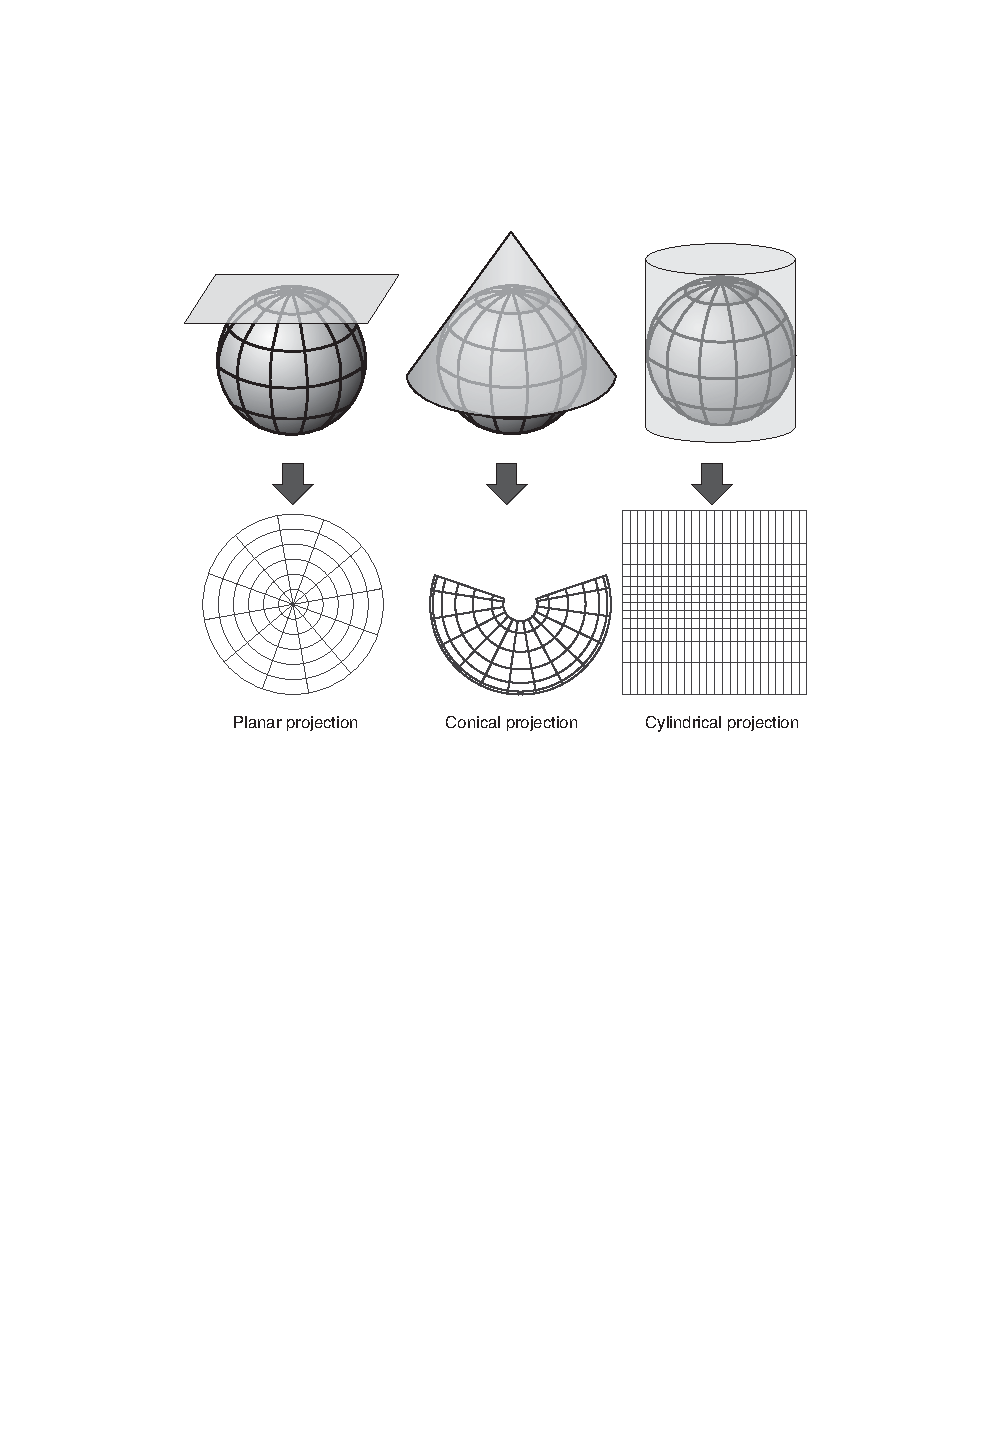
\includegraphics[width=0.75\textwidth]{figures/map_projection_types}
    \caption{Types of map projections~\cite[p 28]{Kupper2005lbs}.}
    \label{fig:map-projection-types}
  \end{center}
\end{figure}

Flattening the curved surface of the Earth naturally causes \textit{distortion} of different kinds, including areal, angular, scale, distance and direction distortion. Selecting a map projection influences which degree and combination of distortion will be caused. As no projection can optimize all those factors at once, choosing the right projection depends on the purpose of the map.

The \textbf{spherical mercator projection} is the most commonly used web mapping projection. Based on a normal cylindrical projection, it preserves local shapes and direction, but does this at the cost of enlarging areas towards the poles. As an example, Greenland appears on a Mercator map larger than South America while its actual size is $1/8$. The effect of this distortion can be visualized by Tissot's indicatrix. Figure \ref{fig:mercator} shows how circles of the same relative size get extrapolated towards the poles when using the mercator projection~\cite{Zzolo11mappingdrupal, wiki:web-mapping, Kupper2005lbs}. 

\begin{figure}[h]
  \begin{center}
    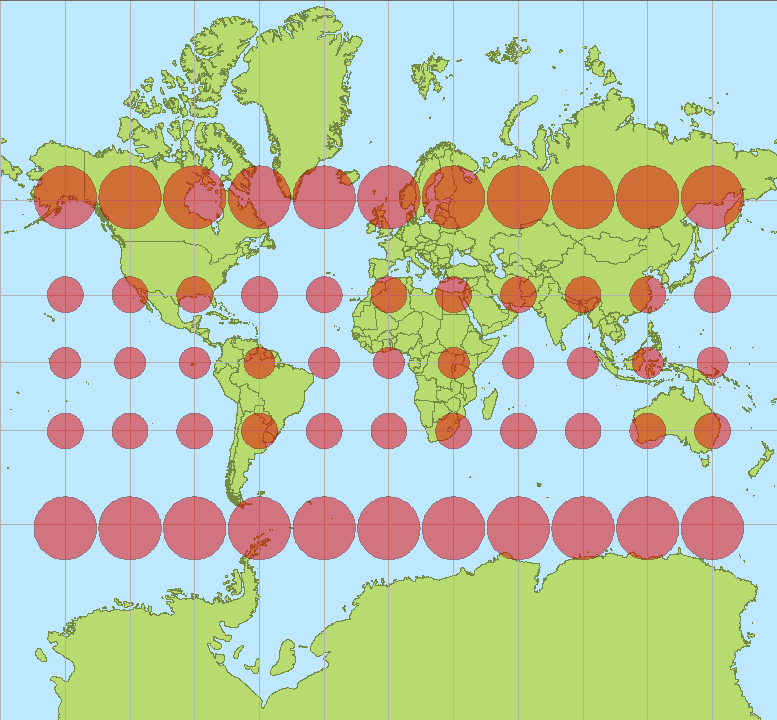
\includegraphics[width=0.65\textwidth]{figures/tissot_mercator.png}
    \caption{Tissot's indicatrix visualizes enlarged areas towards the poles when using the mercator projection~\cite{wiki:mercator}.}
    \label{fig:mercator}
  \end{center}
\end{figure}

Many countries have developed their own coordinate systems, such as the British National Grid or the German Gau\ss-Kr\"{u}ger coordinate system. They aim at reproducing the geographic regions within their territory in an appropriate manner. Standardization efforts go towards using the \textit{Universal Transverse Mercator} projection. It avoids large distortions by comprising a series of Transversal Mercator projections that create separate grid zones with their own projections. This has the benefit of universally representing areas in a more exact way. On the other hand, coordinates need to be referenced including the zones in which they are located in~\cite{Kupper2005lbs}.

\subsection{Spatial data types}

Two main representation types for spatial objects such as buildings, roads and other geometries exist: \textit{vector data} and \textit{raster data}. This mainly applies to 2-dimensional representation of spatial data, which often suffices the task for creating web maps and is preferred over 3-dimensional data handling in many cases for computational simplicity. Figure \ref{fig:raster-vector} illustrates the conceptual different between both data types which will be discussed as follows.

\begin{figure}[h]
  \begin{center}
    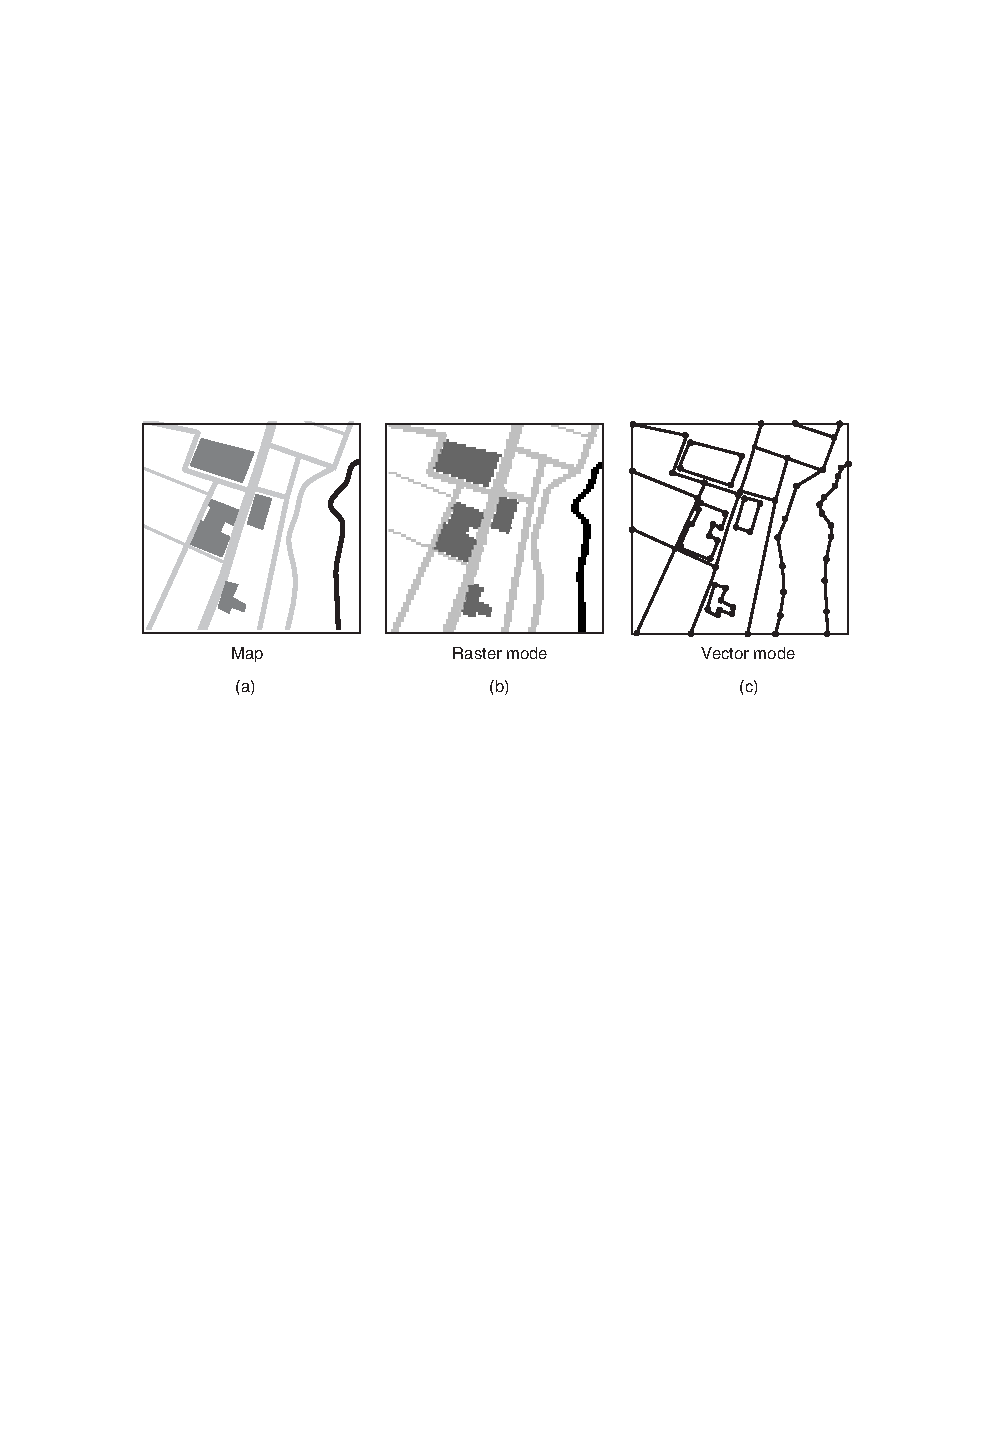
\includegraphics[width=0.9\textwidth]{figures/raster_vs_vector.pdf}
    \caption{A map (a) displayed either in raster mode (b) or in vector mode (c)~\cite[page~38]{Kupper2005lbs}.}
    \label{fig:raster-vector}
  \end{center}
\end{figure}

\begin{itemize}

\item \textbf{Vector data} is used to describe geometric shapes in a numeric way. \textit{Points}, \textit{lines} or \textit{polygons} are specified by coordinates in a reference system.

Simple points can be easily expressed as pairs of latitude, longitude values and stored within two separate columns within a database. More complex shapes like polygons require different data storage types, such as \textit{Well Known Text} (WKT) or \textit{Keyhole Markup Language} (KML).

\item \textbf{Raster data} represents and stores geospatial data as a grid of pixels that forms a continuos surface. It is most commonly used for satellite imaginary. The arrangement of adjacent pixels intrinsically defines the spatial location of shapes within the raster image in relation to an externally defined reference system.

The pixel values of the raster image usually depict a visual representation of the contained area, but they can also be assigned a specific meaning: The \textit{digital elevation model} (DEM) for example is used to describe the average elevation of the mapped area on a per-pixel-basis. Raster images are also often generated from vector data by a tile renderer to create base layers for maps~\cite{Kupper2005lbs, Zzolo11mappingdrupal}.

\end{itemize}








%
% foundations - vis
%

\section{Visualization}

In the following chapter, foundations for visualizing clusters on a map will be discussed. Basics of geographic visualization and their driving forces lead to abstraction and clustering as a tool for simplifying information that needs to be communicated. Visual variables as well as classification approaches for geovisualization will be reviewed in order to review existing concepts for displaying aggregated data on a map.

Visualization is driven by the basic belief that `seeing' is a good way of understanding and generating knowledge. Humans have a very well developed sense of sight, which is underlined by the fact, that more of 50 percent of the neurons in our brain are used in vision.~\cite{vislecture}. 

MacEachren \& Kraak~\cite{maceachren-geovis} define, that ``Geovisualization integrates approaches from visualization in scientific computing (ViSC), cartography, image analysis, information visualization, exploratory data analysis (EDA), and geographic information systems (GISystems) to provide theory, methods, and tools for visual exploration, analysis, synthesis, and presentation of geospatial data (any data having geospatial referencing).'' In his lecture notes on ``Geographic visualization'', Martin N\"{o}llenburg adds that more human-centered definitions exist and observes that the user's needs have to be taken into account for effective geovisualization techniques~\cite{noellenburg11geovis}.


The \textbf{goals of geovisualization} can be summarized using the \textit{map use cube} by MacEachren and Kraak \cite{MacEachren07cartovis}, which is illustrated in figure \ref{fig:geovis-cube}. The goals \textit{exploration, analysis, synthesis and presentation} are classified amongst three dimensions:

\begin{itemize}

\item The type of \textit{task} varies from \textit{knowledge construction} to \textit{information sharing}. While the first is about revealing unknowns and constructing new knowledge, the latter will primarily share existing knowledge.

\item The amount of \textit{interaction} ranges from high to low. A low level of interaction means a rather passive consumption of knowledge, instead a high level will allow the user to actively influence the visualization.

\item The \textit{users} of visualization are classified between public and private audiences. A single, private user might require different visualization techniques than large, public audiences.

\end{itemize}

In the given model of the map use cube, the goals of exploring,analyzing, synthesizing and presenting shift between the extremes of the three defined aspects. The first goal of exploring is classified as a task of knowledge construction, based on high interaction and targeted at a rather private audience. On the other hand, presenting is a task of information sharing that requires a low amount of interaction but is suitable for public audiences~\cite{noellenburg11geovis}.  

\begin{figure}[h]
  \begin{center}
    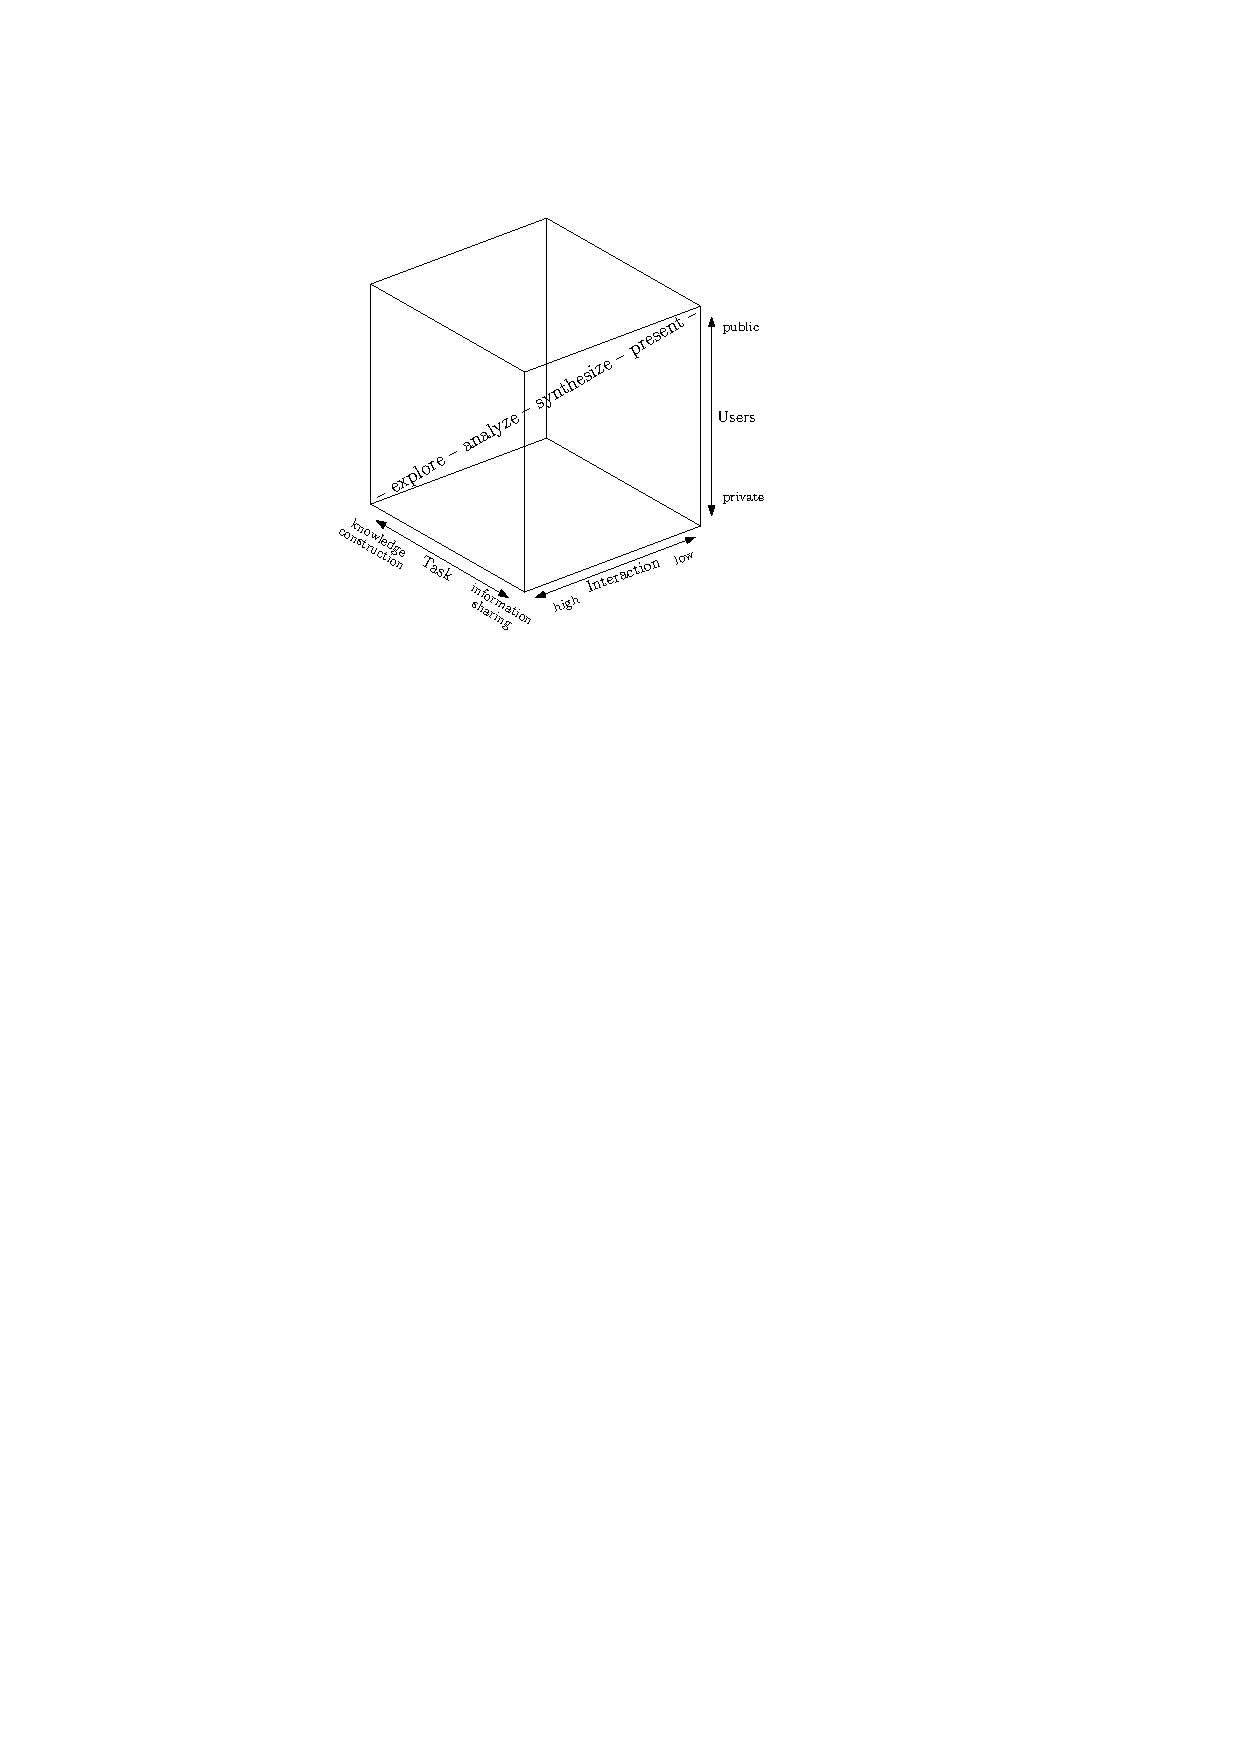
\includegraphics[width=0.65\textwidth]{figures/geovis_goals.pdf}
    \caption{The map use cube after MacEachren and Kraak \cite{MacEachren07cartovis} characterizing geovisualization goals in a three-dimensional space by their level of interaction, their audience, and the addressed tasks.~\cite{noellenburg11geovis}.}
    \label{fig:geovis-cube}
  \end{center}
\end{figure}


Cognitive aspects of visualization help us understand, how visual thinking works. Complex input is abstracted on the retina of the human eye in order to match these abstractions against a vast collection of patterns from experience. Despite generating realistic images, visualization can help generate new ideas by using abstraction to communicate patterns. The idea is to allow the user to join insight, draw conclusions and interact with the data by presenting it in a visual form that reduces the cognitive work needed to perform the given task~\cite{MACEACHREN90apattern, keim2001vis, noellenburg11geovis}. 

Various scientific publications~\cite{phillips82clutter, MACEACHREN90apattern, keim2001vis, harvey2008primer, ellis08clutter, Delort10vis, noellenburg11geovis} that have been researched for this thesis mention the importance of using abstraction for efficiently visualizing information. Especially maps can only highlight interesting information by filtering out unnecessary details of the environment. For example, a road map is better visualized on a clear background instead of satellite images that would distract the user from the primary goal of finding directions. The challenge is to balance realism and abstraction in geovisualization depending on the problem~\cite{noellenburg11geovis}.

\subsection{Visual data exploration techniques}

Depending on the task and the type of data to be shown, different forms of visualization and techniques for exploring the data exist. Daniel A. Keim~\cite{keim2001vis} classifies such techniques using three criteria as depicted in figure \ref{fig:visual-techniques}: the data type to be visualized, the technique itself and the interaction and distortion method~\cite{Delort10vis}:

\begin{itemize}

\item The \textbf{data type} may be one-dimensional (as for example temporal data), two-dimensional (geographical maps), multi-dimensional (relational tables), text and hypertext (articles and web documents), hierarchies and graphs (networks) and algorithms and software (such as debugging operations).

\item The \textbf{visualization techniques} are classified into standard 2d/3d displays (x-y plots and landscapes), geometrically-transformed displays (parallel coordinates), iconic displays (glyphs), dense pixel displays (recursive pattern) and stacked displays (tree maps).

\item Finally, the third dimension describes the \textbf{interaction technique} being used, such as dynamic projection, interactive filtering, zooming, distortion and link \& brush approaches.

\end{itemize}

\begin{figure}[h]
  \begin{center}
    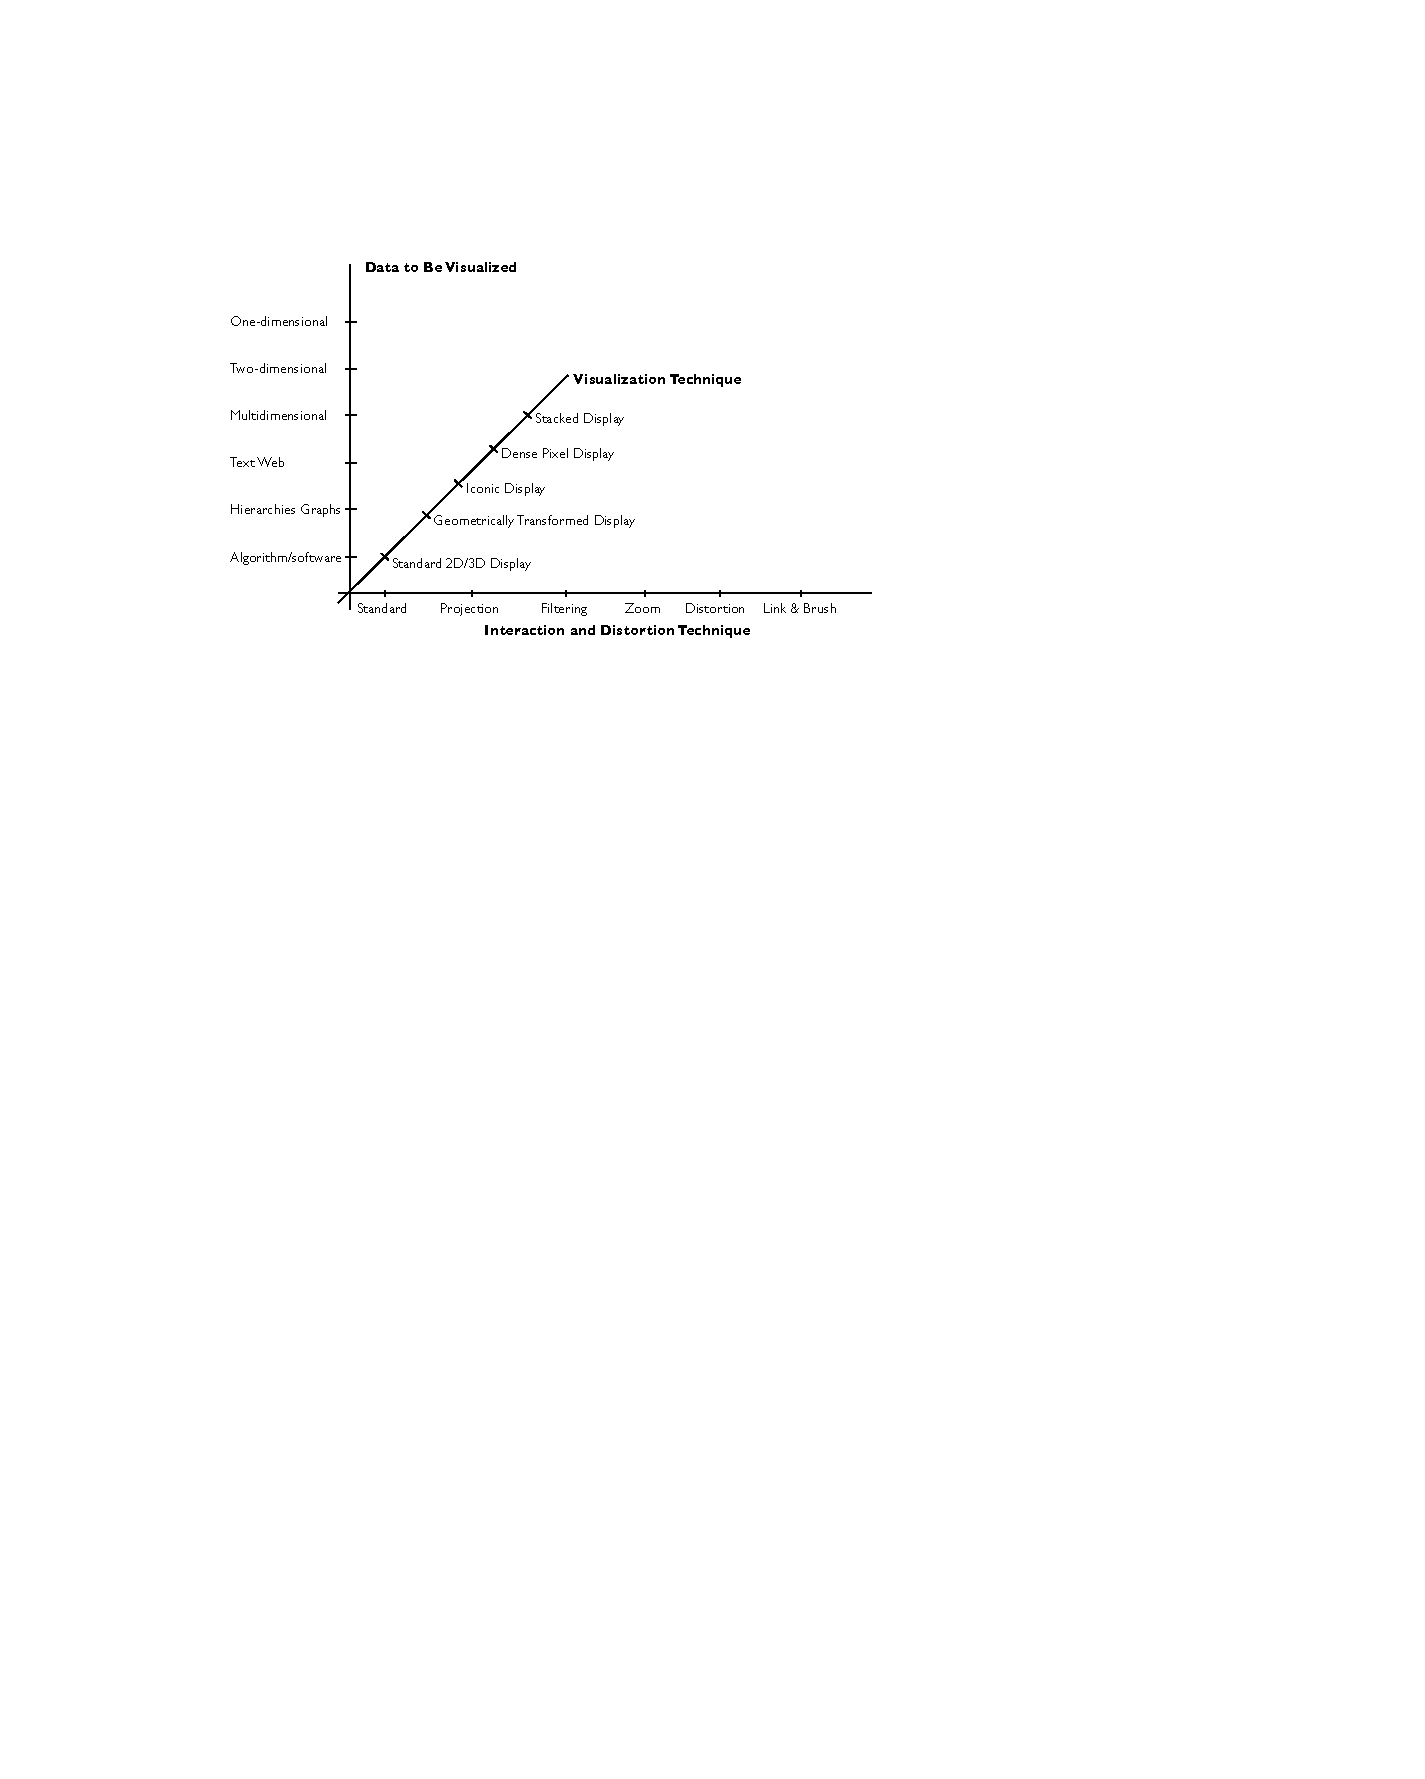
\includegraphics[width=1\textwidth]{figures/classes_visual_techniques.pdf}
    \caption{Classification of visual data exploration techniques based on~\cite{keim2001vis}.}
    \label{fig:visual-techniques}
  \end{center}
\end{figure}


With regard to visualizing clusters on a map, the visualization technique may be considered from two different view points:

\begin{itemize}

\item the visualization of the \textit{entire map} with clustered points on it, as well as

\item the visualization of an \textit{individual cluster}, placed on the map.

\end{itemize}

A map for representing spatially clustered data is based on a least two-dimensional data, containing latitude and longitude information of cluster items. The map is presented in planar space, which classifies it amongst standard 2d/3d displays. Common interaction techniques for maps are zooming and panning which allow to explore the 2-dimensional space and reveal details.

The visualization of individual clusters on the map is likely to be classified amongst iconic displays. During the clustering process, individual points get aggregated, which potentially leads to multivariate aggregate information of item properties. Depending on the level of detail that clusters should expose, more complex visualization techniques may be possible. 

Approaches for visualization techniques of the entire map and individual clusters will be discussed further in chapter TODOREF.

\subsection{Clutter reduction}

Clutter reduction is a way to enhance readability and general performance of maps. An early publication about \textit{visual clutter} on maps by Richard J. Phillips and Liza Noyes~\cite{phillips82clutter} states that ``reducing visual clutter improves map reading performance''. This especially becomes true for visualizing large data sets on maps, so that properties of the data items are hardly visible. Clutter reduces the background visibility and prevents the user from understanding structure and content of the data being presented~\cite{harvey2008primer, Delort10vis}.

Clustering of course is the approach for clutter reduction that is primarily being investigated for this thesis. In order to review the effectiveness and limitations of clustering, as well as the relationship that it has to other techniques in that field, it is helpful to review the ``Clutter Reduction Taxonomy'' by Geoffrey Ellis and Alan Dix~\cite{ellis08clutter}. It distinguishes between three main types of clutter reduction techniques:

\begin{itemize}

\item \textbf{appearance}: alter the look of data items by using techniques like \textit{sampling}, \textit{filtering}, \textit{changing point sizes}, \textit{changing opacity} or \textit{clustering}.

\item \textbf{spatial distortion}: displace the data items in ways as \textit{point/line displacement}, \textit{topological distortion}, \textit{space-filling}, \textit{pixel-plotting} or \textit{dimensional reordering}.

\item \textbf{temporal}: use animation to reveal additional information.

\end{itemize}

In a next step, the stated techniques have been evaluated against a list of 8 high-level criteria. For this thesis, the relevant information for the clustering technique will be outlined for each criterium:

\begin{enumerate}

\item \textit{avoids overlap}
\\ The major benefit is to reduce clutter, provide the ability of seeing and identifying patterns, have less hidden data as well as giving more display space to points. Clustering can be used in such a way to avoid over plotting by representing groups of points as single points.

\item \textit{keeps spatial information}
\\ If a clutter reduction technique maintains the correct coordinates of items is relevant, but the study also states that maintaining relative positions might have greater influence on orientation than just the exact coordinates. Clustering looses the spatial information of individual points, but using aggregate values like the centroid a cluster as the position can be used for compensation. 

\item \textit{can be localized}
\\ The term localization is used to specify, if the display can be reduced to a specific region. This is usually provided by focus and context techniques that reveal information underneath by zooming into an area. The study doesn't make a clear decision regarding the applicability of localization for clustering and states that different properties for spatial and non-spatial clustering apply. In the case of spatial clustering, localization is definitely possible and has been implemented, see chapter \ref{chapter:realization}.  

\item \textit{is scalable}
\\ Scalability of the clutter reduction technique with regards to large amounts of data is the goal of this criterium. The study admits that the meaning of large datasets is vaguely quantified. As one of the main goals for this thesis is to enhance performance for large data set by using clustering, the technique is expected to satisfy this condition. Of course the range of scalability depends on the implemented clustering algorithm. Also refer to the time complexity definitions in chapter \ref{clustering-algorithms}. 

\item \textit{is adjustable}
\\ If the user is able to control aspects of the visual display and adjust parameters of the system that influence the degree of display clutter. Scientific methods in cluster analysis tend to offer a a higher level of interactivity while public facing clustering application limit the amount of interactivity to controlling cluster sizes and the previously discussed localizing feature. 

\item \textit{can show point/line attribute}
\\ The goal is to map attributes of the data to properties like color, shape or opacity of the displayed points or lines. For clustering, this feature can be used in order to display aggregates of the multivariate data results from the clustering process. Further information can be found in chapter TODOREF.

\item \textit{can discriminate points/lines}
\\ Being to able to identify individual data items within a crowded display is the goal of this criterium. The study states the capability of clustering for detecting outliers as well as creating groups of points in order to satisfy this criterion. On the other hand, this classification appear unclear, as the grouping process of clustering hides individual information by definition and only makes it accessible by request or localization. 

\item \textit{can see overlap density}
\\ This helps to gauge the amount of overplotting, see where higher density regions are and understand the distribution of data underlying the visualization. Clustering can show the amount of items within clusters by using visual indicators as point size, opacity and color.  

\end{enumerate}


STATE

\textbf{Driving forces in geovisualization}. The advent of high speed parallel processing and technology advances in computer graphics, today allows us to grasp enormous amounts of information. Besides the advances in graphics and display technologies, the second main driving force in geographic visualization is the increasing amount of geospatial data being collected and available. Finally, the third force is the \textit{rise of the Internet}, which significantly pushes web mapping and contributes to geovisualization technologies~\cite{noellenburg11geovis, vislecture}.

As a logical consequence of broader audiences having access to geospatial visualizations using the Internet, it appears that there is a shift from technology-driven visualization towards more human-centered approaches. 

Glyphs


\begin{figure}[h]
  \begin{center}
    
\includegraphics[width=0.65\textwidth]{figures/glyphs_zame.pdf}
    \caption{Eight different glyphs for aggregated edges (color shade,
average, min/max histogram, min/max range, min/max tribox, Tukey
box, smooth histogram, step histogram)~\cite{ElmqvistDGHF08}.}
    \label{fig:glyphs-zame}
  \end{center}
\end{figure}




